% =====================================================================
%  Rapport de projet Big Data — Niveau de mobilité quotidienne à Dakar
%  Hayat WALDI et Khaoula ELHONNYA — encadré par Pr. BENHLIMA
%  Compilation : XeLaTeX (Overleaf : Menu > Settings > Compiler > XeLaTeX)
% =====================================================================
\documentclass[12pt,a4paper]{report}

% ============================================================
% LANGUE ET TYPOGRAPHIE
% ============================================================
\usepackage{fontspec}
\usepackage{polyglossia}
\setdefaultlanguage{french}
\setmainfont{Latin Modern Roman}
\setsansfont{Latin Modern Sans}
\setmonofont{Latin Modern Mono}[Scale=0.95]
\usepackage{microtype}
\usepackage{setspace}
\onehalfspacing

% ============================================================
% MISE EN PAGE
% ============================================================
\usepackage{geometry}
\geometry{top=2.5cm,bottom=2.5cm,left=3cm,right=2.5cm,headheight=15pt}
\usepackage{fancyhdr}
\usepackage{eso-pic}
\usepackage{enumitem}
\setlist{itemsep=2pt,topsep=4pt}

% ============================================================
% MATHS, TABLEAUX, FIGURES
% ============================================================
\usepackage{amsmath,amssymb}
\usepackage{booktabs,array,tabularx,multirow}
\usepackage{graphicx}
\usepackage{float}
\usepackage{caption}
\usepackage{subcaption}
\usepackage[table]{xcolor}
\usepackage{tikz}
\usetikzlibrary{positioning,arrows.meta,shapes.geometric,calc,fit,backgrounds}
\usepackage[most]{tcolorbox}
\usepackage{listings}
\usepackage{titlesec}
\usepackage{xurl}
\usepackage{hyperref}

% ============================================================
% COULEURS
% ============================================================
\definecolor{ReportBlue}{RGB}{0,66,125}
\definecolor{ReportBlueDark}{RGB}{0,42,85}
\definecolor{ReportBlueLight}{RGB}{222,237,249}
\definecolor{ReportGold}{RGB}{177,139,22}
\definecolor{SoftGray}{RGB}{245,247,250}
\definecolor{TextGray}{RGB}{80,88,97}
\definecolor{CodeGreen}{RGB}{0,120,80}
\definecolor{CodePurple}{RGB}{120,50,150}
% alias utilisés dans le corps du texte
\colorlet{bleu}{ReportBlueDark}
\colorlet{bleuclair}{ReportBlue}
\colorlet{orange}{ReportGold}
\colorlet{gris}{TextGray}

% ============================================================
% IMAGES
% ============================================================
\graphicspath{{./}{./figures/}{./logos/}}

% ============================================================
% INFORMATIONS DU RAPPORT
% ============================================================
\newcommand{\titrecourt}{Prédiction du niveau de mobilité à Dakar -- Rapport de projet Big Data}
\newcommand{\departement}{Département Modélisation et Informatique Scientifique (MIS)}
\newcommand{\annee}{Année universitaire 2026--2027}

% ============================================================
% EN-TÊTES ET PIEDS DE PAGE
% ============================================================
\pagestyle{fancy}
\fancyhf{}
\fancyhead[L]{\small\textcolor{ReportBlue}{\textit{\titrecourt}}}
\fancyhead[R]{\small\textcolor{ReportBlue}{\thepage}}
\fancyfoot[C]{\small\textcolor{TextGray}{\departement}}
\renewcommand{\headrulewidth}{0.5pt}
\renewcommand{\headrule}{\hbox to\headwidth{\color{ReportBlue}\leaders\hrule height \headrulewidth\hfill}}
\fancypagestyle{plain}{%
  \fancyhf{}%
  \fancyhead[R]{\small\textcolor{ReportBlue}{\thepage}}%
  \fancyfoot[C]{\small\textcolor{TextGray}{\departement}}%
  \renewcommand{\headrulewidth}{0pt}}

% ============================================================
% STYLE DES CHAPITRES ET SECTIONS
% ============================================================
\titleformat{\chapter}[display]
  {\normalfont\Large\bfseries\color{ReportBlueDark}}
  {\filleft\large\color{ReportGold}Chapitre \thechapter}
  {1ex}
  {\titlerule[1.4pt]\vspace{1ex}\filright}
  [\vspace{0.8ex}\titlerule]
\titleformat{name=\chapter,numberless}[display]
  {\normalfont\Large\bfseries\color{ReportBlueDark}}
  {}
  {0pt}
  {\titlerule[1.4pt]\vspace{1ex}\filright}
  [\vspace{0.8ex}\titlerule]
\titlespacing*{\chapter}{0pt}{-20pt}{24pt}
\titleformat{\section}{\normalfont\large\bfseries\color{ReportBlueDark}}{\thesection}{0.7em}{}
\titleformat{\subsection}{\normalfont\normalsize\bfseries\color{ReportBlue}}{\thesubsection}{0.6em}{}
\titleformat{\subsubsection}{\normalfont\small\bfseries\color{ReportBlue!80}}{\thesubsubsection}{0.5em}{}

% ============================================================
% LÉGENDES
% ============================================================
\captionsetup{font=small,labelfont={bf,color=ReportBlueDark},labelsep=period,margin=0.8cm}

% ============================================================
% ENCADRÉS
% ============================================================
\newtcolorbox{infobox}{enhanced,colback=ReportBlueLight!55,colframe=ReportBlue,
  boxrule=1.1pt,arc=4pt,left=10pt,right=10pt,top=8pt,bottom=8pt}
\newtcolorbox{constat}[1][À retenir]{enhanced,colback=ReportBlueLight!55,colframe=ReportBlue,
  boxrule=1.1pt,arc=4pt,left=10pt,right=10pt,top=8pt,bottom=8pt,
  coltitle=white,colbacktitle=ReportBlue,fonttitle=\bfseries\small,title=#1}
\newtcolorbox{attention}[1][Point d'attention]{enhanced,colback=ReportGold!9,colframe=ReportGold,
  boxrule=1.1pt,arc=4pt,left=10pt,right=10pt,top=8pt,bottom=8pt,
  coltitle=white,colbacktitle=ReportGold,fonttitle=\bfseries\small,title=#1}

% ============================================================
% STYLE DU CODE
% ============================================================
\lstdefinestyle{pythonstyle}{
  backgroundcolor=\color{SoftGray},
  commentstyle=\color{CodeGreen}\itshape,
  keywordstyle=\color{ReportBlue}\bfseries,
  stringstyle=\color{CodePurple},
  numberstyle=\tiny\color{TextGray},
  basicstyle=\ttfamily\footnotesize,
  breaklines=true, keepspaces=true, columns=fullflexible,
  numbers=left, numbersep=8pt,
  showspaces=false, showstringspaces=false, tabsize=4,
  frame=single, rulecolor=\color{ReportBlue!35},
  language=Python, xleftmargin=15pt, xrightmargin=5pt,
  aboveskip=8pt, belowskip=8pt,
  literate={é}{{\'e}}1 {è}{{\`e}}1 {à}{{\`a}}1 {ê}{{\^e}}1 {É}{{\'E}}1 {→}{{$\rightarrow$}}1 {ô}{{\^o}}1 {ç}{{\c{c}}}1}
\lstset{style=pythonstyle}
\renewcommand{\lstlistingname}{Extrait de code}

% ============================================================
% LIENS
% ============================================================
\hypersetup{colorlinks=true,linkcolor=ReportBlue,urlcolor=ReportBlue,citecolor=ReportGold,
  pdftitle={Prédiction du niveau de mobilité quotidienne à Dakar avec Apache Spark},
  pdfauthor={Hayat WALDI, Khaoula ELHONNYA}}

% ============================================================
% COMMANDES UTILES
% ============================================================
\newcommand{\code}[1]{\texttt{\small #1}}
\newcommand{\1}{\mathbf{1}}
\setlength{\emergencystretch}{3em}

% ============================================================
\begin{document}
% ============================================================

% ============================================================
% PAGE DE GARDE
% ============================================================
\begin{titlepage}
\thispagestyle{empty}
\AddToShipoutPictureBG*{%
  \AtPageUpperLeft{\raisebox{-3.40cm}[0pt][0pt]{\color{ReportBlueDark}\rule{\paperwidth}{3.40cm}}}%
  \AtPageLowerLeft{\raisebox{1.10cm}[0pt][0pt]{\hspace*{1.8cm}\color{ReportBlueDark}\rule{\dimexpr\paperwidth-3.6cm\relax}{1pt}}}%
}
\AddToShipoutPictureFG*{%
  \AtPageUpperLeft{\raisebox{-1.75cm}[0pt][0pt]{\makebox[\paperwidth][c]{%
    \begin{minipage}{0.88\paperwidth}\centering
      {\color{white}\large\bfseries Royaume du Maroc}\\[0.12cm]
      {\color{white}\normalsize Université Mohammed V de Rabat}\\[0.09cm]
      {\color{white}\normalsize École Mohammadia d'Ingénieurs}\\[0.09cm]
      {\color{white}\small \departement}
    \end{minipage}}}}%
}
\centering
\vspace*{1.15cm}

\begin{tabular*}{0.80\textwidth}{@{\extracolsep{\fill}}cc@{}}
  
\includegraphics[height=2.10cm,keepaspectratio]{logos/logoemi.png} &
  
\includegraphics[height=2.00cm,keepaspectratio]{logos/logoum5.png}
\end{tabular*}

\vspace{2cm}

{\LARGE\bfseries\color{ReportBlueDark} RAPPORT DE PROJET}

\vspace{0.18cm}
{\normalsize Module : Big Data -- Cycle Ingénieur}

\vspace{0.55cm}
{\normalsize Apache Spark · PySpark · Spark SQL · MLlib}

\vspace{1.2cm}
\begin{tikzpicture}
\node[draw=ReportBlue,rounded corners=5pt,line width=1.1pt,fill=ReportBlueLight!22,
      text width=0.78\textwidth,inner xsep=16pt,inner ysep=15pt,align=center]{%
  {\LARGE\bfseries\color{ReportBlueDark} Prédiction du niveau de mobilité\\[0.08cm] quotidienne à Dakar}

  \vspace{0.22cm}
  {\large\itshape Exploratory Data Analysis et Machine Learning\\ distribué avec Apache Spark}
};
\end{tikzpicture}

\vspace{1.8cm}
\noindent\hspace*{0.75cm}%
\begin{minipage}[t]{0.40\textwidth}\raggedright
\textbf{\color{ReportBlueDark}Réalisé par :}\\[0.12cm]
Hayat WALDI\\
Khaoula ELHONNYA
\end{minipage}\hfill
\begin{minipage}[t]{0.42\textwidth}\raggedright
\textbf{\color{ReportBlueDark}Encadré par :}\\[0.12cm]
Pr. BENHLIMA\\[0.42cm]
\textbf{\color{ReportBlueDark}Données :}\\[0.12cm]
Enquête ménages-déplacements, Dakar
\end{minipage}

\vfill
{\large\bfseries\color{ReportBlueDark} \annee}

\vspace{0.45cm}
\end{titlepage}

% ============================================================
% REMERCIEMENTS
% ============================================================
\pagenumbering{roman}
\chapter*{Remerciements}
\addcontentsline{toc}{chapter}{Remerciements}

Nous tenons à remercier sincèrement \textbf{Pr. BENHLIMA} pour son enseignement dans le cadre du module Big Data, ainsi que pour ses conseils et sa disponibilité tout au long de ce projet. Ce travail nous a permis de mettre en pratique, sur des données réelles, les notions de traitement distribué, de Spark SQL et de Machine Learning avec Spark MLlib abordées en cours.

Nous remercions également l'\textbf{École Mohammadia d'Ingénieurs} et le \textbf{\departement} pour le cadre de formation qui a rendu ce projet possible.

% ============================================================
% RÉSUMÉ
% ============================================================
\chapter*{Résumé}
\addcontentsline{toc}{chapter}{Résumé}

\begin{infobox}
Ce rapport présente un projet de Big Data mené sur l'enquête ménages-déplacements de la région de Dakar : à partir du profil d'une personne et de son ménage, nous cherchons à prédire son \textbf{niveau de mobilité quotidienne} (peu mobile, mobile ou très mobile) à l'aide d'Apache Spark et de Spark MLlib.
\end{infobox}

Les 45\,605 déplacements fournis (33 variables) ont d'abord fait l'objet d'une \textbf{Exploratory Data Analysis (EDA)} avec pandas : contrôle de la qualité (heures codées au-delà de minuit, coût codé \code{99999}, codes de zone spéciaux), distributions, outliers, bivariate analysis et correlations. Ses conclusions ont guidé la construction d'une \textbf{chaîne de traitement distribuée} avec Spark : ingestion avec schéma explicite, nettoyage, agrégation des déplacements en 11\,457 individus, variables de ménage calculées par window functions, statistiques pondérées en Spark SQL, puis modélisation avec Spark MLlib (Logistic Regression, Decision Tree, Random Forest). Les données sont découpées par ménage en \textbf{train, validation et test sets (70 / 15 / 15\,\%)} : le validation set sert à comparer les modèles et à régler leurs hyperparameters, et le test set n'est utilisé qu'une seule fois, pour l'évaluation finale.

L'étude montre qu'un Dakarois mobile effectue en moyenne \textbf{3,9 déplacements par jour}, que les jeunes, les élèves, les hommes et les habitants de la banlieue (Rufisque, Guédiawaye) sont les plus mobiles, et que 88\,\% des individus font un nombre pair de déplacements (logique d'allers-retours). Le modèle retenu, un \textbf{Random Forest}, atteint sur le test set (ménages jamais vus) une \textbf{accuracy de 44,7\,\%}, contre 36,1\,\% pour la baseline, un score très proche de celui obtenu sur le validation set (45,1\,\%). Ce gain modeste montre que le profil socio-démographique n'explique qu'une partie de la mobilité ; l'absence de variables comme le revenu, la profession, la motorisation ou les distances en est la principale limite.

\vspace{0.35cm}
\noindent\textbf{Mots-clés :} Big Data ; Apache Spark ; PySpark ; Spark SQL ; MLlib ; mobilité urbaine ; Dakar ; multiclass classification ; EDA ; data leakage ; Machine Learning.

\clearpage
\tableofcontents
\clearpage
\listoffigures
\addcontentsline{toc}{chapter}{Liste des figures}
\clearpage
\listoftables
\addcontentsline{toc}{chapter}{Liste des tableaux}
\clearpage
\pagenumbering{arabic}

% ============================================================
% INTRODUCTION GÉNÉRALE
% ============================================================
\chapter*{Introduction générale}
\addcontentsline{toc}{chapter}{Introduction générale}

La région de Dakar concentre près d'un quart de la population du Sénégal et l'essentiel de son activité économique. Sa croissance rapide, portée par l'extension de la banlieue (Pikine, Guédiawaye, Rufisque), pose de forts enjeux de mobilité : accès à l'emploi, à l'école et aux services, saturation des axes vers le centre, et place prépondérante de la marche et des transports collectifs artisanaux (cars rapides, Ndiaga Ndiaye, Tata).

Les enquêtes ménages-déplacements sont l'outil de référence pour comprendre ces pratiques : elles décrivent, pour chaque membre d'un échantillon de ménages, l'ensemble des déplacements réalisés au cours d'une journée. Le \emph{taux de mobilité}, c'est-à-dire le nombre de déplacements par personne et par jour, y est un indicateur central : il mesure l'accès effectif d'un individu aux opportunités de la ville.

Ce projet, réalisé dans le cadre du module Big Data, exploite un extrait de cette enquête. Il pose la problématique suivante :

\vspace{0.35cm}
\begin{center}
\begin{tikzpicture}
\node[draw=ReportBlue,fill=ReportBlueLight,rounded corners=5pt,text width=13cm,
      align=center,inner sep=0.45cm,line width=1.1pt]{%
  \textbf{\large Problématique}\\[0.22cm]
  \itshape À partir des caractéristiques d'une personne, de la composition de son ménage et de sa zone de résidence, peut-on prédire son niveau de mobilité quotidienne, et quels facteurs la déterminent le plus~?
};
\end{tikzpicture}
\end{center}
\vspace{0.35cm}

Contrairement à une approche par déplacement (prédire le mode, le motif ou la durée d'un trajet), ce projet se place \textbf{au niveau de l'individu}. Il faut donc transformer les données par agrégation, une opération typique des traitements Big Data. Les objectifs sont les suivants :
\begin{enumerate}[leftmargin=*]
  \item réaliser une \textbf{EDA} (Exploratory Data Analysis) complète pour évaluer la qualité des données et identifier les déterminants de la mobilité ;
  \item construire une \textbf{chaîne de traitement distribuée} avec Apache Spark : ingestion, nettoyage, agrégation et ingénierie des variables ;
  \item produire des \textbf{statistiques pondérées} représentatives de la population ;
  \item entraîner, optimiser et évaluer des \textbf{modèles de classification} avec Spark MLlib, puis en interpréter les résultats.
\end{enumerate}

Le chapitre~\ref{ch:donnees} présente les données et le chapitre~\ref{ch:methodo} décrit la méthodologie et l'architecture technique. Le chapitre~\ref{ch:eda} détaille l'EDA, le chapitre~\ref{ch:spark} la préparation des données avec Spark et le chapitre~\ref{ch:modele} la modélisation. Les résultats sont présentés au chapitre~\ref{ch:resultats} et discutés au chapitre~\ref{ch:discussion}, avant la conclusion générale.

% ============================================================
% CHAPITRE 1 — DONNÉES
% ============================================================
\chapter{Présentation des données}\label{ch:donnees}

\section{Source et structure}
Les données sont fournies sous la forme d'un classeur Excel ({\small\nolinkurl{donnees_deplacement_PSpark_2026.xlsx}}) de quatre feuilles :

\begin{table}[H]
\centering
\caption{Contenu du classeur fourni}\label{tab:feuilles}
\begin{tabularx}{\linewidth}{@{}lX@{}}
\toprule
\textbf{Feuille} & \textbf{Contenu} \\
\midrule
\code{deplacement} & Table principale : une ligne par déplacement (45\,605 lignes, 33 colonnes). \\
\code{matrice\_OD} & Tableau croisé dynamique origine–destination pondéré par strate. \\
\code{explication} & Dictionnaire partiel des variables. \\
\code{strate\_commune} & Correspondance entre les codes de strate et les 52 communes. \\
\bottomrule
\end{tabularx}
\end{table}

\section{Variables}
L'unité statistique de la table \code{deplacement} est le \textbf{déplacement}, c'est-à-dire le fait de se rendre d'une origine à une destination pour un motif donné, éventuellement en plusieurs trajets. Les 33 variables se répartissent en six familles (tableau~\ref{tab:variables}).

\begin{table}[H]
\centering
\caption{Familles de variables de la table \code{deplacement}}\label{tab:variables}
\small
\begin{tabularx}{\linewidth}{@{}lX@{}}
\toprule
\textbf{Famille} & \textbf{Variables} \\
\midrule
Identifiants & \code{numMena}, \code{num\_individu}, \code{num\_Deplacement} \\
Spatiales & \code{LieuDepart}, \code{Origine\_StrateDepart}, \code{LieuArrivee}, \code{Dextination\_StrateArrivee} \\
Temporelles & \code{HeureDepart}, \code{HeureArrivee} (format HHMM), \code{Duree (mn)}, \code{JourEnqueteIndi} \\
Individu & \code{Age}, \code{Sexe}, \code{PositMenage} \\
Déplacement & \code{Motif}, \code{NbTrajets}, \code{Mode1}…\code{Mode4}, \code{NbTrajets*} (10 colonnes), \code{Cout}, \code{Moyen de transport} \\
Pondération & \code{Poids\_extra} (poids d'extrapolation) \\
\bottomrule
\end{tabularx}
\end{table}

\section{Volumétrie et unité d'analyse}
Le fichier décrit \textbf{45\,605 déplacements} réalisés par \textbf{11\,457 individus} de \textbf{3\,127 ménages}, âgés de 11 à 95 ans. La variable \code{Poids\_extra} indique combien de déplacements réels chaque ligne représente : sa somme estime à environ \textbf{6,7 millions} le nombre de déplacements quotidiens dans la population.

Notre question portant sur les personnes, l'unité d'analyse du modèle est l'\textbf{individu} : les données doivent donc être agrégées (chapitre~\ref{ch:spark}).


\section{Synthèse du chapitre}
Le jeu de données décrit 45\,605 déplacements, réalisés par 11\,457 individus de 3\,127 ménages et décrits par 33 variables. L'unité statistique d'origine est le déplacement ; notre question portant sur les personnes, les données devront être agrégées au niveau de l'individu.

% ============================================================
% CHAPITRE 3 — MÉTHODOLOGIE
% ============================================================
\chapter{Méthodologie et architecture}\label{ch:methodo}

\section{Démarche générale}
Le projet suit une démarche classique de science des données, adaptée au contexte Big Data : l'exploration se fait sur un échantillon en mémoire (pandas), tandis que la préparation et la modélisation sont implémentées avec Spark, de façon à pouvoir passer à l'échelle sans modification du code.

\begin{figure}[H]
\centering
\begin{tikzpicture}[
  node distance=0.55cm and 0.5cm,
  etape/.style={rectangle,rounded corners=3pt,draw=bleuclair,fill=bleu!5,text width=2.55cm,
                minimum height=1.25cm,align=center,font=\sffamily\scriptsize},
  cle/.style={etape,fill=orange!12,draw=orange},
  fleche/.style={-{Stealth[length=2.2mm]},thick,bleuclair}]
  \node[etape] (xlsx) {\textbf{Excel}\\ 4 feuilles};
  \node[etape,right=of xlsx] (eda) {\textbf{EDA}\\ pandas};
  \node[etape,right=of eda] (ingest) {\textbf{Ingestion}\\ CSV + schéma\\ explicite, \code{cache()}};
  \node[etape,right=of ingest] (clean) {\textbf{Nettoyage}\\ Spark SQL};
  \node[cle,below=of clean] (agg) {\textbf{Agrégation}\\ \code{groupBy}\\ déplacements \(\rightarrow\) personnes};
  \node[etape,left=of agg] (win) {\textbf{Variables ménage}\\ window functions};
  \node[etape,left=of win] (ml) {\textbf{Spark MLlib}\\ Pipeline,\\ train / valid. / test};
  \node[etape,left=of ml] (out) {\textbf{Résultats}\\ évaluation,\\ prédictions};
  \draw[fleche] (xlsx) -- (eda);
  \draw[fleche] (eda) -- (ingest);
  \draw[fleche] (ingest) -- (clean);
  \draw[fleche] (clean) -- (agg);
  \draw[fleche] (agg) -- (win);
  \draw[fleche] (win) -- (ml);
  \draw[fleche] (ml) -- (out);
  \node[font=\sffamily\scriptsize\color{gris},above=2pt of eda] {Partie 1};
  \node[font=\sffamily\scriptsize\color{gris},above=2pt of ingest] {Partie 2 (Spark)};
\end{tikzpicture}
\caption{Chaîne de traitement du projet}\label{fig:pipeline}
\end{figure}

\section{Environnement technique}
\begin{table}[H]
\centering
\caption{Environnement logiciel}\label{tab:env}
\begin{tabular}{@{}ll@{}}
\toprule
\textbf{Composant} & \textbf{Version / configuration} \\
\midrule
Apache Spark (PySpark) & 3.5.3, mode \code{local[*]} \\
Système & Windows (Anaconda, JupyterLab) \\
Java & OpenJDK 17 (Eclipse Temurin) \\
Python & 3 (Anaconda) avec pandas, NumPy, Matplotlib, Seaborn \\
Partitions de shuffle & \code{spark.sql.shuffle.partitions = 8} \\
Mémoire du driver & 4 Go \\
Stockage des tables & En mémoire avec \code{cache()} \\
\bottomrule
\end{tabular}
\end{table}

\begin{attention}[Exécution sous Windows]
Le notebook a été exécuté sous Windows. Pour que Spark fonctionne, nous avons configuré Java (\code{JAVA\_HOME}), conservé les tables intermédiaires en mémoire avec \code{cache()} au lieu de les écrire sur le disque, et utilisé uniquement des fonctions Spark natives. Les modèles sont entraînés l'un après l'autre pour respecter la mémoire disponible.
\end{attention}

\section{Pourquoi Spark~?}
Le jeu de données tient en mémoire, mais une enquête de ce type peut être répétée sur plusieurs années, étendue à d'autres villes ou enrichie de traces GPS. Les choix techniques visent donc la \textbf{scalabilité} :
\begin{itemize}
  \item \textbf{mise en cache} (\code{cache()}) : les tables réutilisées restent en mémoire et ne sont pas recalculées à chaque étape ;
  \item \textbf{transformations distribuées} (\code{groupBy}, fenêtres, jointures) : aucune donnée n'est rapatriée sur le driver, sauf les petits résultats agrégés destinés aux graphiques ;
  \item \textbf{MLlib} : pipelines reproductibles (préparation + modèle), entraînés de façon distribuée.
\end{itemize}


\section{Synthèse du chapitre}
Le projet combine une exploration en mémoire avec pandas et une chaîne de traitement Spark conçue pour passer à l'échelle.

% ============================================================
% CHAPITRE 4 — EDA
% ============================================================
\chapter{Exploratory Data Analysis (EDA)}\label{ch:eda}

L'EDA est menée avec pandas, d'abord au niveau des déplacements (qualité des données), puis au niveau des personnes (target et déterminants).

\section{Qualité des données}

\subsection{Missing values et doublons}
Seules cinq variables présentent des valeurs manquantes (figure~\ref{fig:manquants}). Les colonnes \code{Mode2} à \code{Mode4} ne sont renseignées que lorsque le déplacement compte plusieurs trajets : leur vacuité est \textbf{structurelle} et ne doit pas être imputée. \code{Cout} (11 lignes) et \code{NbTrajetsAPied} (1 ligne) sont marginales. Aucun doublon n'existe sur la clé (ménage, individu, numéro de déplacement).

\begin{figure}[H]
\centering
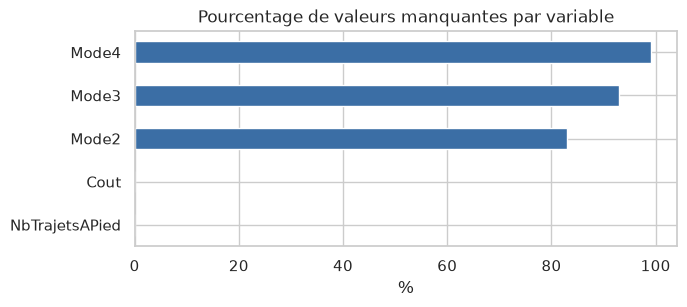
\includegraphics[width=0.62\linewidth]{cell9.png}
\caption{Pourcentage de valeurs manquantes par variable}\label{fig:manquants}
\end{figure}

\subsection{Anomalies et outliers}
Les statistiques descriptives et les boxplots (figure~\ref{fig:aberrants}) révèlent plusieurs anomalies, résumées dans le tableau~\ref{tab:anomalies}.

\begin{figure}[H]
\centering
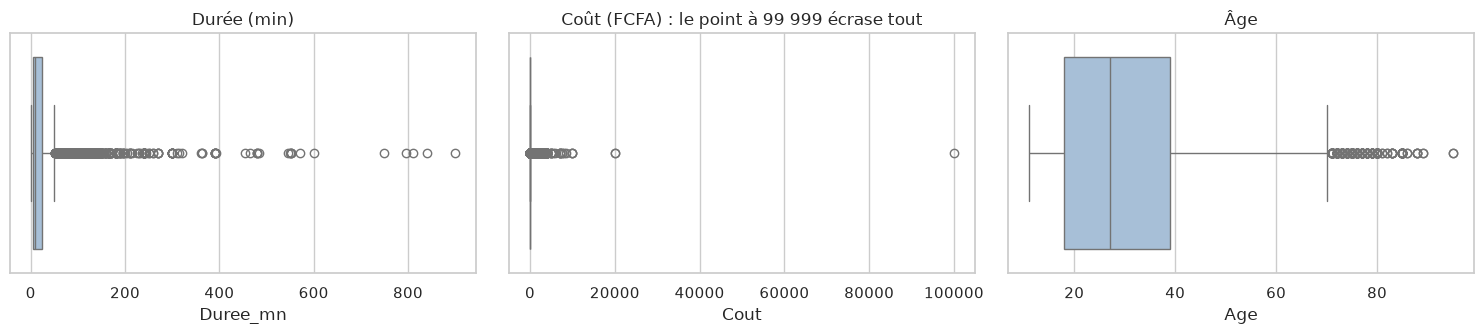
\includegraphics[width=\linewidth]{cell21.png}
\caption{Boxplots de la durée, du coût et de l'âge}\label{fig:aberrants}
\end{figure}

\begin{table}[H]
\centering
\caption{Anomalies détectées et traitement retenu}\label{tab:anomalies}
\small
\begin{tabularx}{\linewidth}{@{}Xrl@{}}
\toprule
\textbf{Anomalie} & \textbf{Lignes} & \textbf{Traitement} \\
\midrule
Coût codé \code{99999} (« inconnu ») & 1 & remplacé par \code{null} \\
Heure de départ \(\geq 2400\) (après minuit, format HHMM) & 270 & heure ramenée sur 0--23 h pour l'analyse \\
Durée supérieure à 3 heures & 83 & conservée (compte comme déplacement) \\
Codes de strate spéciaux (\code{zex}, \code{NA\_d}, \code{NA\_p}…) & 519 & règle dédiée pour le département \\
Durée incohérente avec les heures (écart \(> 5\) min) & 0 & aucun \\
\bottomrule
\end{tabularx}
\end{table}

\begin{attention}
La règle de l'IQR (InterQuartile Range) signale plus de 3\,000 « outliers » pour la durée et plus de 10\,000 pour le coût. Il s'agit en réalité de distributions très \textbf{asymétriques} (marche gratuite et courte contre transports collectifs longs et payants), et non d'erreurs. Seules les anomalies du tableau~\ref{tab:anomalies} sont traitées.
\end{attention}

\section{Distributions des variables}
La figure~\ref{fig:distrib} présente les distributions des principales variables numériques. La population enquêtée est jeune (âge médian de 27 ans). Les durées sont courtes (médiane de 10 minutes) avec une longue traîne. Les départs se concentrent autour de trois pics (7~h, 10~h et 17--19~h). 77\,\% des déplacements sont gratuits, et 83\,\% se font en un seul trajet.

\begin{figure}[H]
\centering
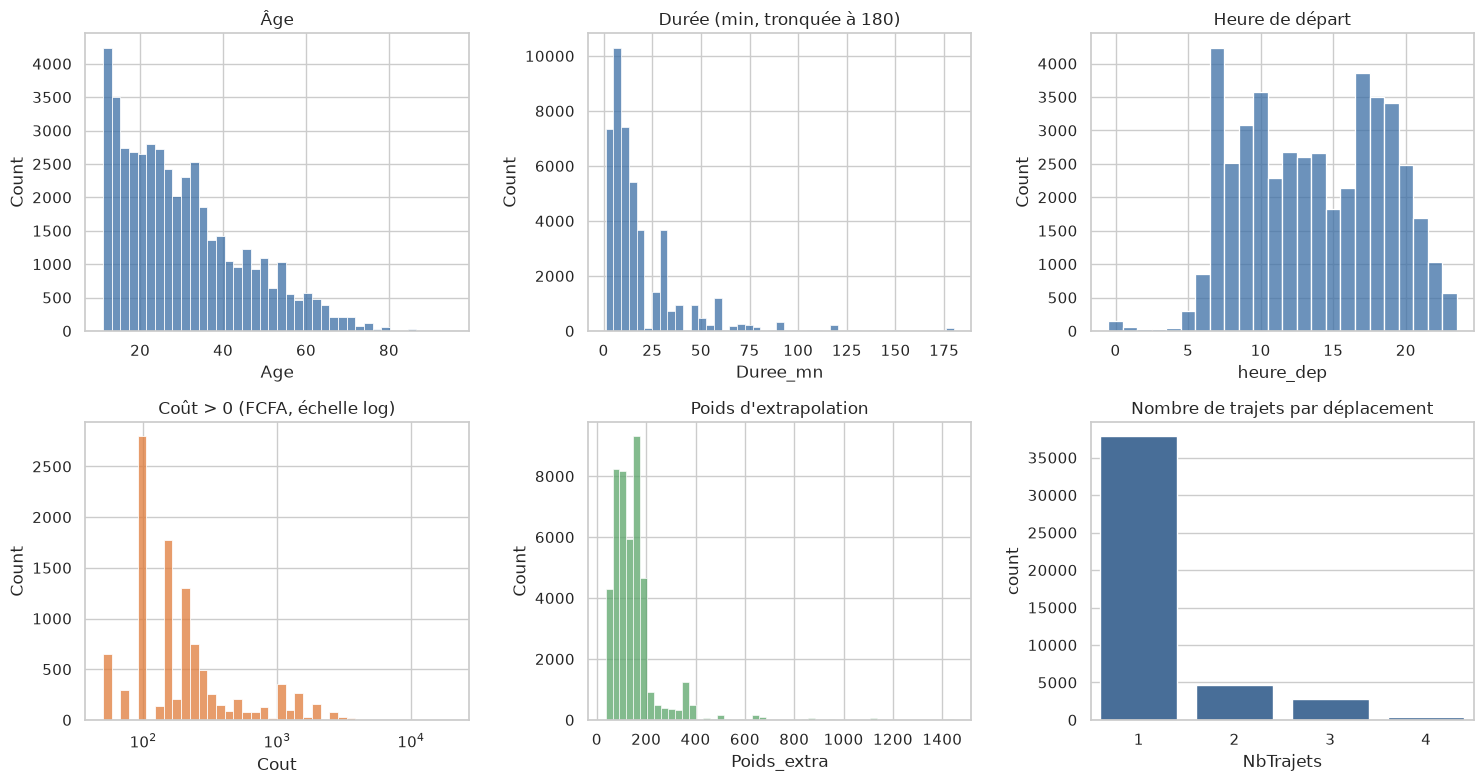
\includegraphics[width=\linewidth]{cell17.png}
\caption{Distributions des variables numériques}\label{fig:distrib}
\end{figure}

Les variables catégorielles (figure~\ref{fig:categ}) confirment la prédominance de la marche (70\,\% des déplacements) et du motif « retour au domicile » (43\,\%). L'échantillon est équilibré entre hommes (50,7\,\%) et femmes (49,3\,\%) ; le lundi n'est pas enquêté.

\begin{figure}[H]
\centering
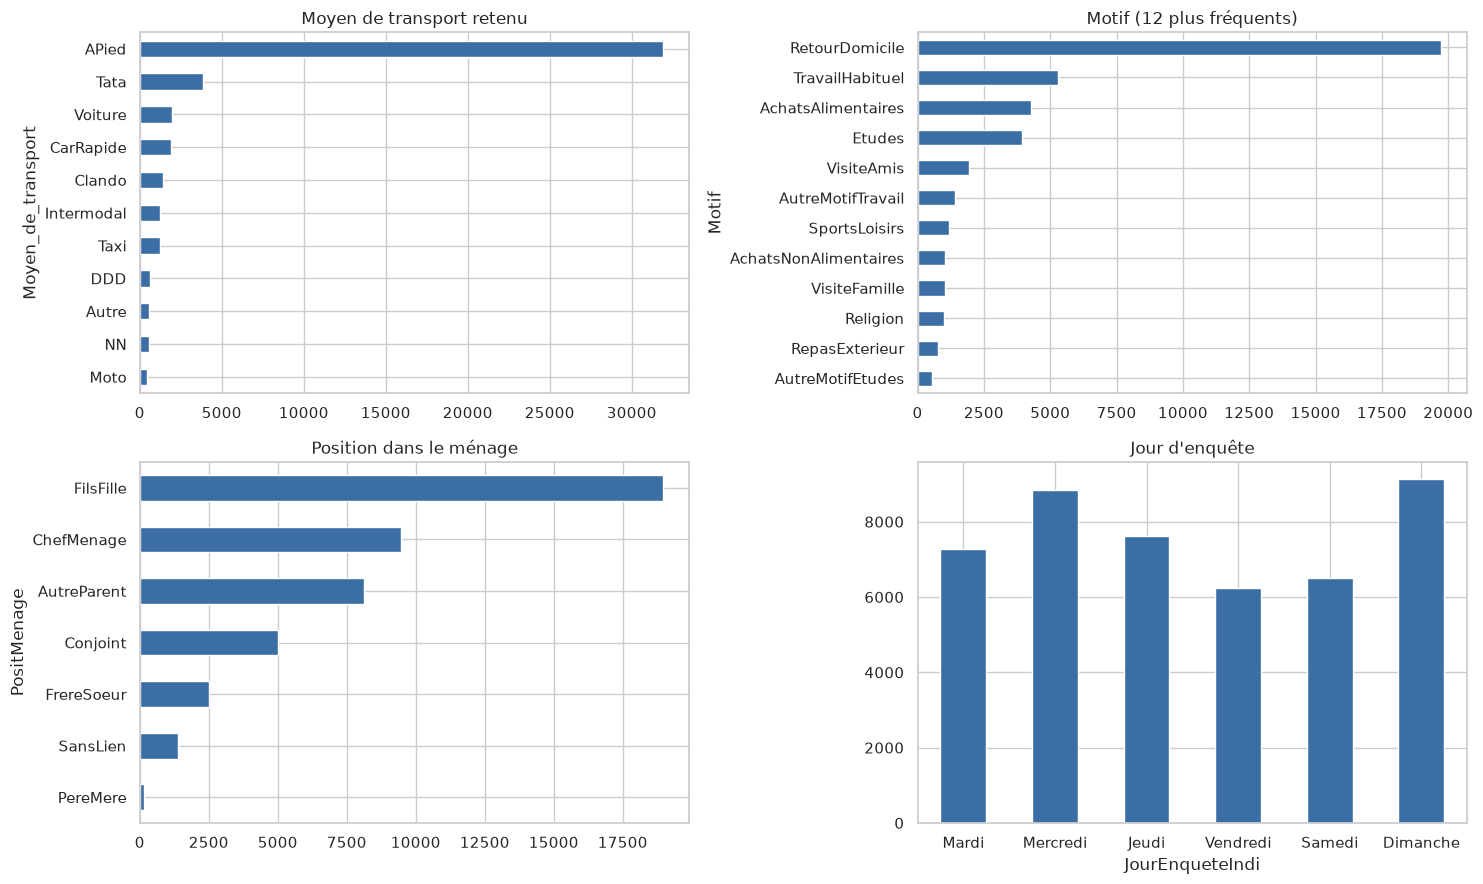
\includegraphics[width=\linewidth]{cell24.png}
\caption{Distribution des principales variables catégorielles}\label{fig:categ}
\end{figure}

\section{Le rythme d'une journée}
Pour comprendre concrètement ce qu'est un déplacement, la figure~\ref{fig:rythme} montre à quelle heure on part selon le motif, et la figure~\ref{fig:journee} reconstitue la journée réelle d'un élève de l'enquête.

\begin{figure}[H]
\centering
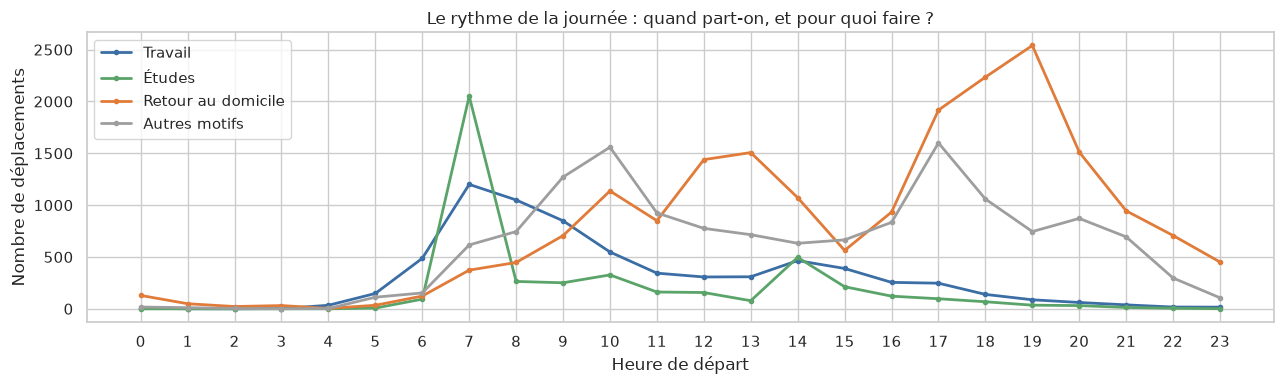
\includegraphics[width=\linewidth]{fig_rythme.png}
\caption{Nombre de départs par heure selon la famille de motifs}\label{fig:rythme}
\end{figure}

\begin{figure}[H]
\centering
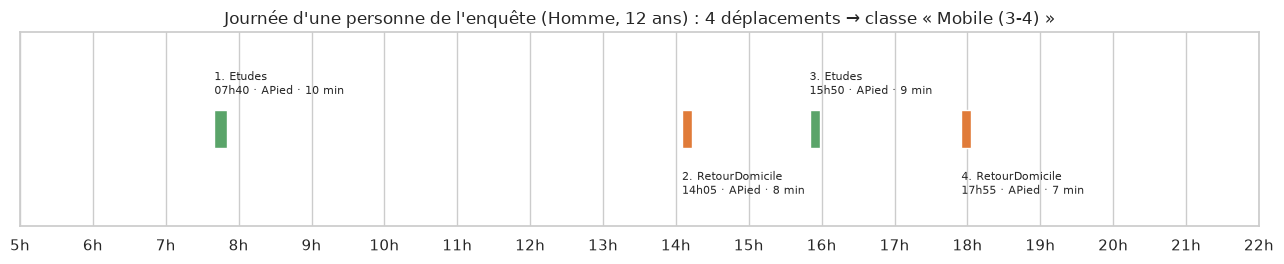
\includegraphics[width=\linewidth]{fig_journee.png}
\caption{Journée d'un élève de 12 ans de l'enquête : quatre déplacements}\label{fig:journee}
\end{figure}

Les départs pour les études et le travail culminent à 7~h ; les retours au domicile forment deux pics, vers 12--13~h (retour pour le déjeuner) et vers 19~h. La journée de l'élève suit la logique des \textbf{allers-retours} : domicile \(\rightarrow\) école \(\rightarrow\) domicile, deux fois dans la journée, soit 4 déplacements. Le dernier déplacement ramène la personne chez elle, ce qui permettra de connaître sa zone de résidence.

\section{Passage au niveau individu et target}
Les déplacements sont regroupés par individu, et l'on compte leur nombre dans la journée. Le nombre moyen est de \textbf{4 déplacements} par personne (médiane 4, maximum 18).

La figure~\ref{fig:cible} met en évidence un phénomène remarquable : \textbf{88\,\% des individus effectuent un nombre pair de déplacements}, ce qui traduit la logique des allers-retours depuis le domicile. De plus, 98\,\% des journées se terminent par un retour au domicile, ce qui permet de déduire la \textbf{zone de résidence} comme la strate d'arrivée du dernier déplacement.

\begin{figure}[H]
\centering
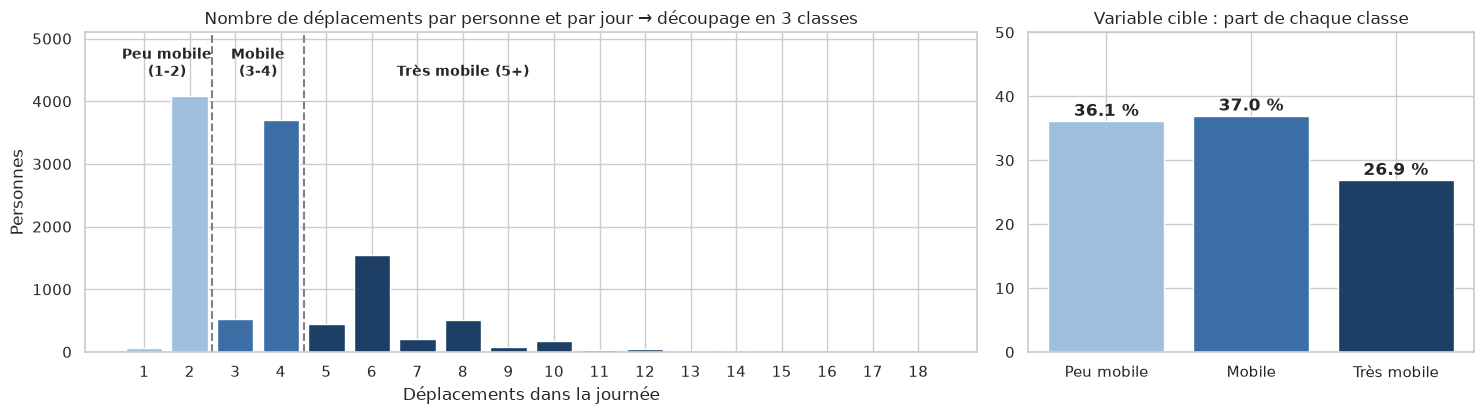
\includegraphics[width=\linewidth]{fig_cible.png}
\caption{Nombre de déplacements par personne, découpé en trois classes (à gauche), et part de chaque classe (à droite)}\label{fig:cible}
\end{figure}

La target est définie en trois classes, dont les effectifs sont équilibrés :

\begin{table}[H]
\centering
\caption{Définition de la target}\label{tab:cible}
\begin{tabular}{@{}clcc@{}}
\toprule
\textbf{Code} & \textbf{Niveau de mobilité} & \textbf{Déplacements / jour} & \textbf{Part des individus} \\
\midrule
0 & Peu mobile & 1 -- 2 & 36,1\,\% \\
1 & Mobile & 3 -- 4 & 37,0\,\% \\
2 & Très mobile & 5 et plus & 26,9\,\% \\
\bottomrule
\end{tabular}
\end{table}

\begin{attention}[Limite de la target]
L'enquête ne contient que des personnes s'étant déplacées au moins une fois. Le modèle prédit donc l'\textbf{intensité} de la mobilité, et non le fait de se déplacer ou non.
\end{attention}

\section{Bivariate analysis}
La figure~\ref{fig:bivariee} croise le nombre moyen de déplacements avec les principales caractéristiques des individus.

\begin{figure}[H]
\centering
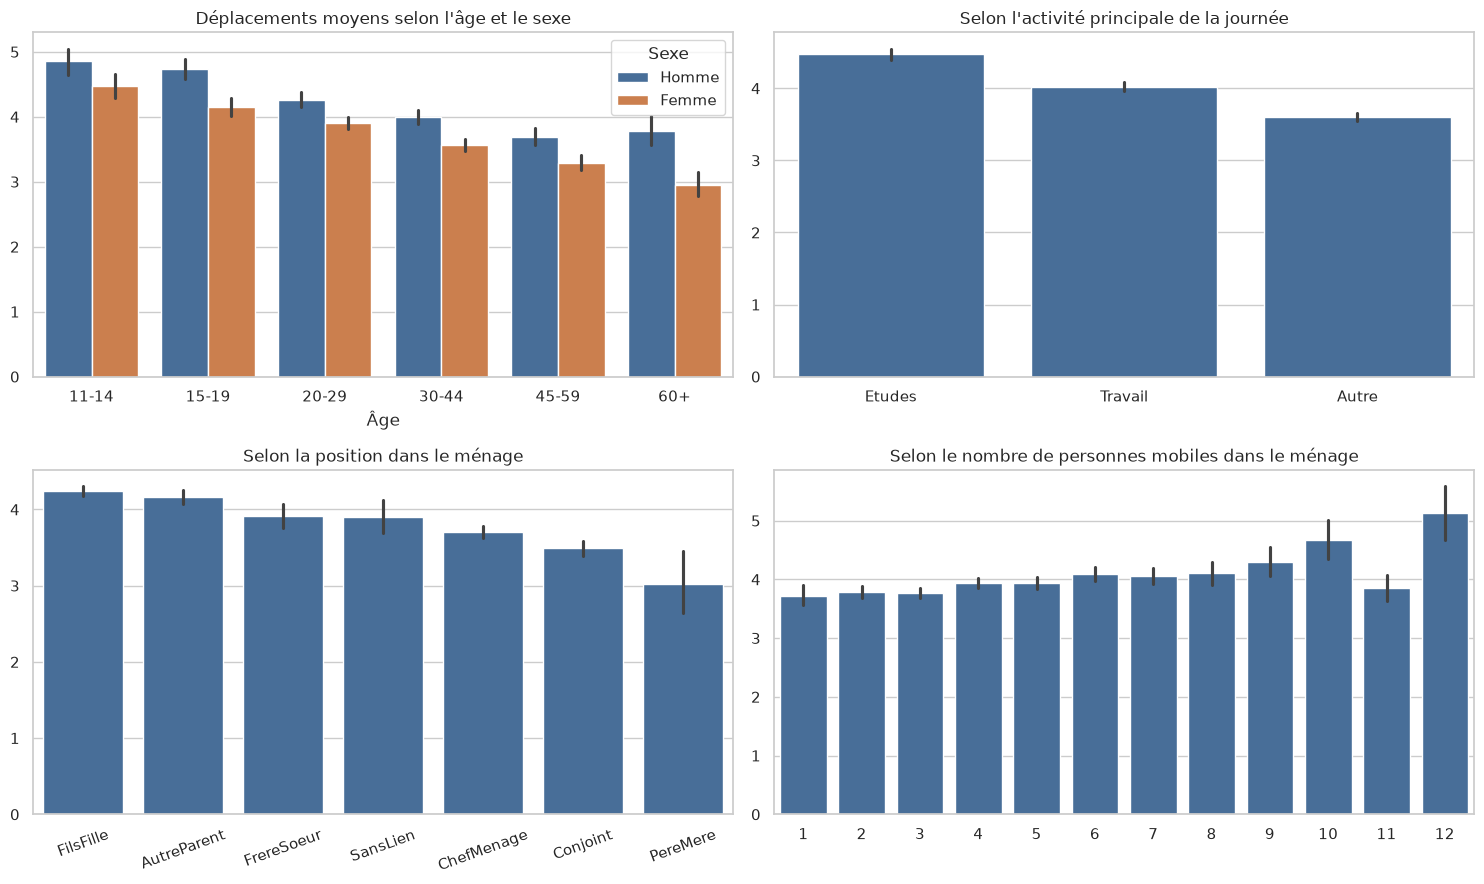
\includegraphics[width=\linewidth]{cell33.png}
\caption{Nombre moyen de déplacements selon l'âge et le sexe, l'activité, la position dans le ménage et la taille du ménage}\label{fig:bivariee}
\end{figure}

\begin{constat}[Déterminants de la mobilité]
\begin{itemize}[leftmargin=*]
  \item \textbf{Âge} : facteur le plus net. Les 11--14 ans font 4,65 déplacements par jour contre 3,46 après 60 ans (allers-retours scolaires, souvent matin et après-midi).
  \item \textbf{Activité} : élèves et étudiants (4,47) $>$ actifs (4,02) $>$ autres (3,60).
  \item \textbf{Sexe} : hommes 4,20 contre femmes 3,78.
  \item \textbf{Ménage} : la mobilité individuelle croît avec le nombre de personnes mobiles du ménage (de 3,7 à 4,7).
  \item \textbf{Jour} : effet quasi nul (3,9 à 4,1).
\end{itemize}
\end{constat}

Les moyennes cachent la répartition. La figure~\ref{fig:composition} montre, pour chaque groupe, la part de peu mobiles, de mobiles et de très mobiles.

\begin{figure}[H]
\centering
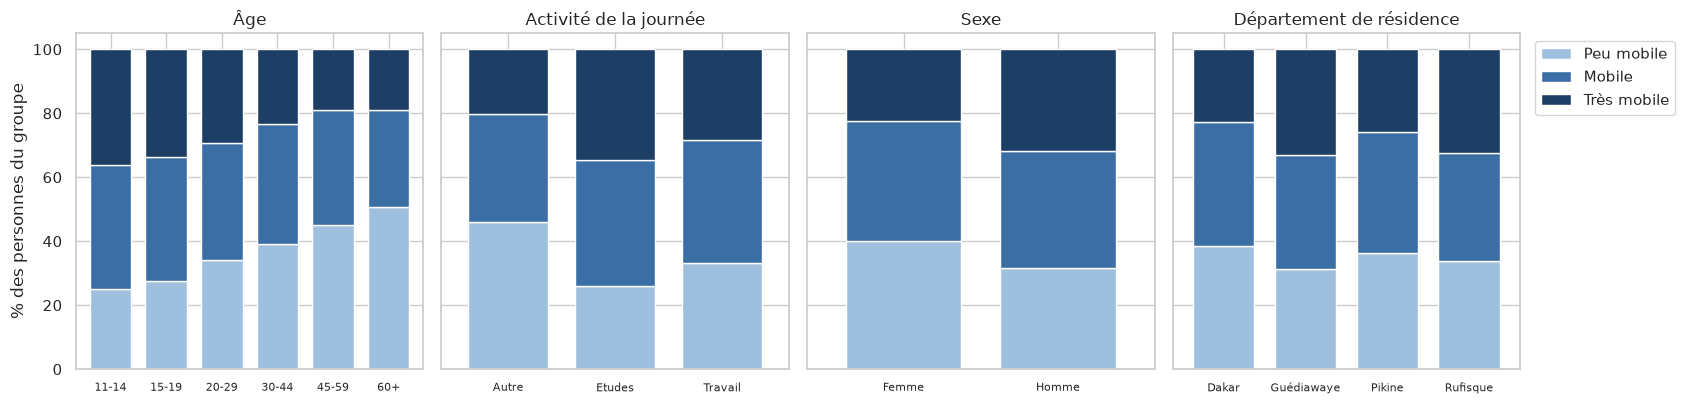
\includegraphics[width=\linewidth]{fig_composition.png}
\caption{Composition des classes de mobilité selon l'âge, l'activité, le sexe et le département}\label{fig:composition}
\end{figure}

La part de très mobiles baisse avec l'âge et est la plus forte chez les élèves ; la part de peu mobiles est la plus forte après 60 ans et chez les personnes sans travail ni études ce jour-là. Mais \textbf{dans chaque groupe, les trois classes sont présentes} : aucun profil n'est « toujours très mobile », ce qui annonce une prédiction difficile.

\section{Correlation matrix}
Aucune variable n'est fortement corrélée, prise seule, au nombre de déplacements (\(|r| < 0{,}2\), figure~\ref{fig:corr}). La mobilité résulte d'une \textbf{combinaison} de facteurs, ce qui justifie de comparer plusieurs modèles multivariés, linéaires (Logistic Regression) et non linéaires (Decision Tree, Random Forest). La corrélation ne mesure toutefois que les liens linéaires entre variables numériques : les variables catégorielles, comme la zone de résidence, n'y apparaissent pas.

\begin{figure}[H]
\centering
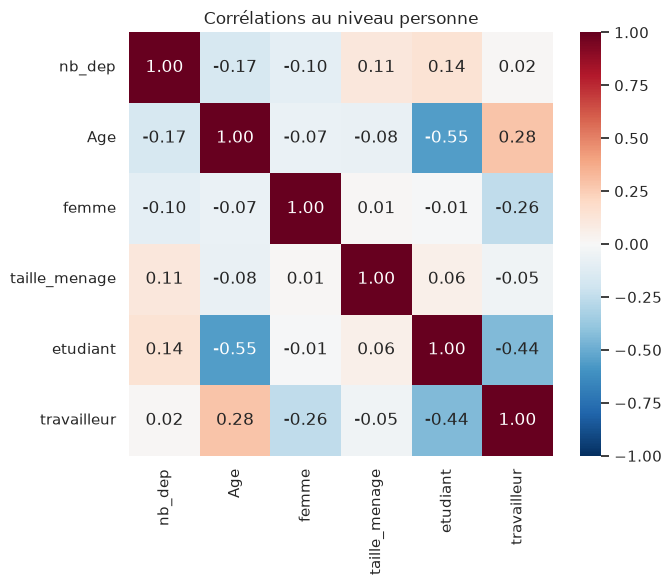
\includegraphics[width=0.55\linewidth]{cell38.png}
\caption{Correlation matrix au niveau individu}\label{fig:corr}
\end{figure}

\begin{attention}[Data leakage]
On obtiendrait des corrélations bien plus fortes avec des variables calculées sur la journée (nombre de motifs différents, durée totale, coût total, modes utilisés). Mais elles sont calculées à partir des \textbf{mêmes déplacements} que la target : elles augmentent mécaniquement avec le nombre de déplacements et contiennent donc déjà la réponse. Elles sont \textbf{exclues} des features.
\end{attention}

\section{Synthèse du chapitre : du constat à la décision}
\begin{table}[H]
\centering
\caption{Décisions de préparation issues de l'EDA}\label{tab:decisions}
\small
\begin{tabularx}{\linewidth}{@{}XX@{}}
\toprule
\textbf{Constat} & \textbf{Décision appliquée dans Spark} \\
\midrule
Heures HHMM, coût \code{99999}, durées \(> 3\) h & Coût codé \(\rightarrow\) \code{null}, heures converties en minutes ; déplacements longs conservés \\
La question porte sur les individus & Agrégation \code{groupBy(numMena, num\_individu)} \\
98\,\% des journées finissent au domicile & Résidence = strate d'arrivée du dernier déplacement \\
Classes équilibrées (36 / 37 / 27\,\%) & Target en 3 classes, accuracy et F1-score comme métriques \\
Influence de la composition du ménage & Variables de ménage par window functions \\
Activité fortement liée à la mobilité & Deux scénarios : profil seul (A) et profil + activité (B) \\
Individus d'un même ménage corrélés & Split train / validation / test (70 / 15 / 15) \textbf{par ménage} \\
\code{Poids\_extra} constant par individu & Statistiques pondérées à l'échelle de la population \\
\bottomrule
\end{tabularx}
\end{table}


% ============================================================
% CHAPITRE 5 — SPARK
% ============================================================
\chapter{Préparation des données avec Apache Spark}\label{ch:spark}

\section{Session Spark}
La session Spark est le point d'entrée de tout le traitement. Elle est lancée en mode local sur tous les cœurs du processeur (\code{local[*]}), avec 8 partitions après les regroupements et 4~Go de mémoire.

\begin{lstlisting}[caption={Création de la session Spark},label={lst:session}]
spark = (SparkSession.builder
         .appName("Mobilite_Quotidienne_Dakar")
         .master("local[*]")
         .config("spark.sql.shuffle.partitions", "8")
         .config("spark.driver.memory", "4g")
         .getOrCreate())
\end{lstlisting}

\section{Ingestion}
Spark ne disposant pas de lecteur natif pour le format \code{.xlsx}, la feuille \code{deplacement} est convertie une seule fois en CSV, puis lue par Spark avec un \textbf{schéma explicite} (33 champs typés). Un schéma explicite évite le double parcours des données qu'impose \code{inferSchema} et garantit les types. La table est ensuite mise en cache pour ne pas relire le fichier à chaque calcul.

\begin{lstlisting}[caption={Lecture du CSV avec un schéma explicite},label={lst:ingestion}]
dep_pd = pd.read_excel(file, sheet_name="deplacement")
dep_pd.columns = [c.replace(" (mn)", "_mn").replace(" ", "_") for c in dep_pd.columns]
dep_pd.to_csv("data/raw/deplacement.csv", index=False)

df = spark.read.csv("data/raw/deplacement.csv", header=True, schema=schema).cache()
\end{lstlisting}

\section{Contrôles de qualité}
Les contrôles de l'EDA sont reproduits en Spark, de façon distribuée : absence de doublons, 1 coût codé, 270 départs après minuit et 83 déplacements de plus de 3 heures. On vérifie en outre que l'âge, le sexe, le jour et le poids sont \textbf{constants pour chaque individu}, condition nécessaire pour agréger sans perte d'information.

\section{Nettoyage}
Le nettoyage applique les décisions de l'EDA : le coût codé \code{99999} est remplacé par une valeur vide, les heures de départ au format HHMM sont converties en minutes depuis minuit et ramenées sur 0--24~h, et deux indicateurs (0 ou 1) repèrent les déplacements effectués pour le travail et pour les études. Une fonction calcule aussi le département à partir du code de zone, en traitant les codes spéciaux (voir l'annexe).

\begin{lstlisting}[caption={Nettoyage des déplacements},label={lst:nettoyage}]
clean = (df
    .withColumn("Cout", F.when(F.col("Cout") >= 99999, None).otherwise(F.col("Cout")))
    .withColumn("heure_dep_min",
                ((F.col("HeureDepart") / 100).cast("int") * 60 + F.col("HeureDepart") % 100) % 1440)
    .withColumn("est_travail", F.col("Motif").isin(motifs_travail).cast("int"))
    .withColumn("est_etudes", F.col("Motif").isin(motifs_etudes).cast("int"))
).cache()
\end{lstlisting}

La figure~\ref{fig:nettoyage} compare les données brutes et nettoyées.

\begin{figure}[H]
\centering
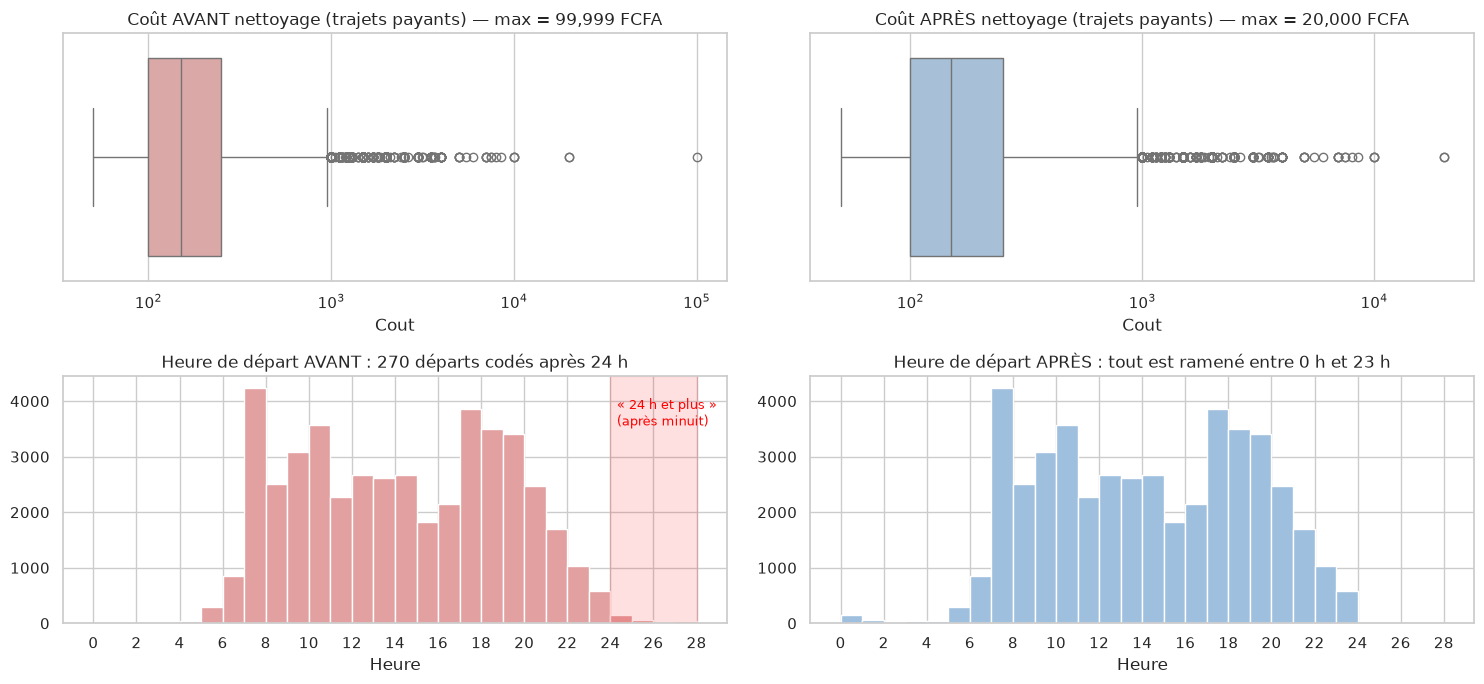
\includegraphics[width=\linewidth]{fig_nettoyage.png}
\caption{Coût et heure de départ avant et après nettoyage}\label{fig:nettoyage}
\end{figure}

Avant nettoyage, le code \code{99999} étirait toute la distribution du coût ; après, le maximum est de 20\,000~FCFA, un coût plausible pour un long trajet en taxi. Les 270 départs codés après « 24~h » sont ramenés au petit matin. Le nettoyage est \textbf{léger} : il ne supprime aucune ligne et ne modifie pas la target.

\section{Agrégation des déplacements en individus}
C'est l'étape clé du projet. Un \code{groupBy} distribué transforme les 45\,605 déplacements en 11\,457 individus. La fonction \code{max\_by} récupère la strate d'arrivée du dernier déplacement (zone de résidence), et des indicateurs de motif déterminent l'activité principale de la journée.

\begin{lstlisting}[caption={Agrégation distribuée au niveau individu},label={lst:agg}]
personnes = (clean.groupBy("numMena", "num_individu")
    .agg(F.count("*").alias("nb_dep"),
         F.first("Age").alias("Age"), F.first("Sexe").alias("Sexe"),
         F.first("PositMenage").alias("PositMenage"),
         F.first("JourEnqueteIndi").alias("Jour"),
         F.first("Poids_extra").alias("poids"),
         F.max_by("Dextination_StrateArrivee", "num_Deplacement")
          .alias("strate_residence"),
         F.max("est_travail").alias("va_travail"),
         F.max("est_etudes").alias("va_etudes"))
    .withColumn("activite", F.when(F.col("va_travail") == 1, "Travail")
                             .when(F.col("va_etudes") == 1, "Etudes")
                             .otherwise("Autre")))
\end{lstlisting}

Le tableau~\ref{tab:exemple_menage} illustre cette transformation sur un ménage réel de trois personnes : ses 12 déplacements deviennent 3 lignes, une par personne.

\begin{table}[H]
\centering
\caption{Un ménage avant et après l'agrégation (ménage n\textsuperscript{o}~2)}\label{tab:exemple_menage}
\small
\begin{tabular}{@{}cccll@{\hspace{1cm}}ccc@{}}
\toprule
\multicolumn{5}{c}{\textbf{Avant : déplacements}} & \multicolumn{3}{c}{\textbf{Après : personnes}} \\
\cmidrule(r){1-5}\cmidrule(l){6-8}
\textbf{Indiv.} & \textbf{N\textsuperscript{o}} & \textbf{Heure} & \textbf{Motif} & \textbf{Arrivée} & \textbf{Indiv.} & \textbf{\code{nb\_dep}} & \textbf{Activité} \\
\midrule
1 & 1 & 9h15 & TravailHabituel & D01 & \multirow{4}{*}{1} & \multirow{4}{*}{4} & \multirow{4}{*}{Travail} \\
1 & 2 & 10h30 & RepasExterieur & D01 & & & \\
1 & 3 & 18h00 & TravailHabituel & D01 & & & \\
1 & 4 & 19h15 & RetourDomicile & D01 & & & \\
\midrule
2 & 1 & 8h00 & AutreMotifTravail & D17 & \multirow{4}{*}{2} & \multirow{4}{*}{4} & \multirow{4}{*}{Travail} \\
2 & 2 & 13h30 & Religion & D02 & & & \\
2 & 3 & 15h10 & VisiteAmis & D04 & & & \\
2 & 4 & 19h00 & RetourDomicile & D01 & & & \\
\midrule
3 & 1 & 8h00 & TravailHabituel & D04 & \multirow{4}{*}{3} & \multirow{4}{*}{4} & \multirow{4}{*}{Travail} \\
3 & 2 & 16h15 & Associations & D06 & & & \\
3 & 3 & 16h30 & AutreMotifMenage & D04 & & & \\
3 & 4 & 19h20 & RetourDomicile & D01 & & & \\
\bottomrule
\end{tabular}
\end{table}

\section{Variables du ménage par window functions}
Une fenêtre partitionnée par ménage calcule des statistiques collectives et les recopie sur chaque membre, sans jointure ni collecte sur le driver. Contrairement à un \code{groupBy}, le nombre de lignes ne change pas : dans le ménage n\textsuperscript{o}~2, les trois membres gardent leur ligne et reçoivent les mêmes valeurs de ménage (taille 3, âge moyen 28,3 ans, aucune femme).

\begin{lstlisting}[caption={Variables de ménage calculées par window functions},label={lst:fenetre}]
w_menage = Window.partitionBy("numMena")
personnes = (personnes
    .withColumn("taille_menage", F.count("*").over(w_menage))
    .withColumn("nb_enfants", F.sum((F.col("Age") < 18).cast("int")).over(w_menage))
    .withColumn("nb_seniors", F.sum((F.col("Age") >= 60).cast("int")).over(w_menage))
    .withColumn("nb_adultes", F.col("taille_menage") - F.col("nb_enfants") - F.col("nb_seniors"))
    .withColumn("age_moyen_menage", F.round(F.avg("Age").over(w_menage), 1))
    .withColumn("part_femmes_menage", F.round(F.avg((F.col("Sexe") == "Femme").cast("int")).over(w_menage), 2))
    .withColumn("sexe_chef", F.coalesce(
        F.max(F.when(F.col("PositMenage") == "ChefMenage", F.col("Sexe"))).over(w_menage), F.lit("Inconnu")))
    .withColumn("weekend", F.col("Jour").isin("Samedi", "Dimanche").cast("int"))
    .withColumn("niveau", F.when(F.col("nb_dep") <= 2, 0).when(F.col("nb_dep") <= 4, 1).otherwise(2).cast("double"))
)
personnes = personnes.cache()
\end{lstlisting}

\section{Statistiques pondérées avec Spark SQL}
Le poids d'extrapolation permet d'estimer la mobilité de l'ensemble de la population. La population mobile de 11 ans et plus est estimée à \textbf{1,70 million} de personnes, qui réalisent \textbf{6,70 millions} de déplacements par jour, soit \textbf{3,93 déplacements} par personne.

\begin{table}[H]
\centering
\caption{Mobilité pondérée selon le sexe, l'activité et le département de résidence}\label{tab:ponderees}
\small
\begin{tabular}{@{}llrrrr@{}}
\toprule
\textbf{Variable} & \textbf{Modalité} & \textbf{Effectif} & \textbf{Dépl./jour} & \textbf{\% peu mobiles} & \textbf{\% très mobiles} \\
\midrule
\multirow{2}{*}{Sexe} & Homme & 5\,514 & 4,16 & 32,1 & 31,2 \\
 & Femme & 5\,943 & 3,72 & 41,4 & 21,5 \\
\midrule
\multirow{3}{*}{Activité} & Études & 2\,950 & 4,41 & 26,6 & 33,4 \\
 & Travail & 4\,231 & 3,99 & 33,7 & 27,9 \\
 & Autre & 4\,276 & 3,55 & 47,0 & 19,6 \\
\midrule
\multirow{4}{*}{Département} & Rufisque & 2\,430 & 4,29 & 35,2 & 32,3 \\
 & Guédiawaye & 1\,156 & 4,23 & 30,8 & 31,9 \\
 & Pikine & 3\,742 & 3,93 & 37,4 & 25,7 \\
 & Dakar & 4\,117 & 3,73 & 38,4 & 23,1 \\
\bottomrule
\end{tabular}
\end{table}

\begin{figure}[H]
\centering
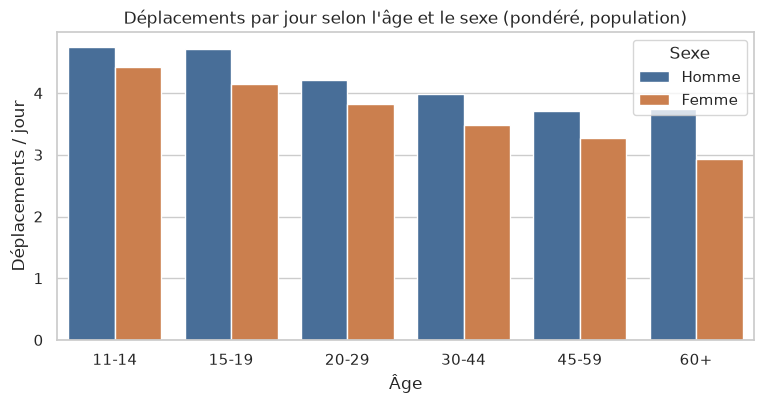
\includegraphics[width=0.72\linewidth]{cell58.png}
\caption{Déplacements par jour selon l'âge et le sexe (estimation pondérée)}\label{fig:ponderee}
\end{figure}

L'écart entre hommes et femmes existe à tout âge et s'accentue avec l'âge : il est le plus marqué après 60 ans (environ 3,7 déplacements par jour pour les hommes contre 2,9 pour les femmes), puis chez les 15--19 ans. Enfin, près d'une personne sur deux sans activité de travail ou d'études dans la journée (47\,\%) est peu mobile, contre 27\,\% des élèves et étudiants.

\section{Synthèse du chapitre}
Spark transforme les 45\,605 déplacements en 11\,457 individus enrichis de variables de ménage, sans rapatrier les données sur le driver. Les estimations pondérées confirment les écarts observés pendant l'exploration : les jeunes, les élèves, les hommes et les habitants de la banlieue sont les plus mobiles.

% ============================================================
% CHAPITRE 6 — MODÉLISATION
% ============================================================
\chapter{Modélisation avec Spark MLlib}\label{ch:modele}

\section{Features}
\begin{table}[H]
\centering
\caption{Features du modèle}\label{tab:features}
\small
\begin{tabularx}{\linewidth}{@{}l>{\raggedright\arraybackslash}X>{\raggedright\arraybackslash}p{5.2cm}@{}}
\toprule
\textbf{Type} & \textbf{Variables} & \textbf{Encodage} \\
\midrule
Catégorielles & Sexe, position dans le ménage, jour, strate et département de résidence, sexe du chef de ménage & \code{StringIndexer} (+ \code{OneHotEncoder}) \\
Numériques & Âge, taille du ménage, nombres d'enfants, d'adultes et de seniors, âge moyen du ménage, part de femmes, week-end & valeurs brutes (standardisées pour la Logistic Regression) \\
Scénario B & Activité principale de la journée (travail, études, autre) & \code{StringIndexer} \\
\bottomrule
\end{tabularx}
\end{table}

\section{Deux scénarios}
\begin{itemize}[leftmargin=*]
  \item \textbf{Scénario A -- profil seul} : uniquement des informations connues avant la journée.
  \item \textbf{Scénario B -- profil + activité} : ajout de l'activité principale, qui sert d'indicateur du statut de la personne (élève, actif). Cette variable n'étant pas déclarée dans l'enquête, elle est déduite des motifs de la journée ; le scénario B constitue donc une borne optimiste.
\end{itemize}

\section{Train / validation / test split}
Les membres d'un même ménage partagent des habitudes et les mêmes variables de ménage. Si une personne était dans un jeu et un membre de sa famille dans un autre, le modèle aurait déjà « vu » ce ménage et son score serait trop optimiste (data leakage). Le découpage se fait donc \textbf{par ménage}, à partir d'un hash de l'identifiant du ménage ramené entre 0 et 99 : tous les membres d'un ménage tombent dans le même jeu.

\begin{table}[H]
\centering
\caption{Rôle et taille des trois jeux}\label{tab:split}
\small
\resizebox{\linewidth}{!}{%
\begin{tabular}{@{}llrrl@{}}
\toprule
\textbf{Jeu} & \textbf{Buckets} & \textbf{Personnes} & \textbf{Ménages} & \textbf{Rôle} \\
\midrule
Train set & 0--69 & 8\,087 (70,6\,\%) & 2\,224 & entraîner les modèles \\
Validation set & 70--84 & 1\,710 (14,9\,\%) & 449 & comparer les modèles, choisir les hyperparameters \\
Test set & 85--99 & 1\,660 (14,5\,\%) & 454 & évaluer une seule fois le modèle final \\
\bottomrule
\end{tabular}}
\end{table}

Trois jeux sont nécessaires : si le meilleur modèle était choisi en regardant le test set, il finirait par s'y adapter et son score serait trop optimiste. Le validation set sert à \textbf{faire les choix} ; le test set reste \textbf{intact} jusqu'à la fin. La figure~\ref{fig:split} vérifie que les trois jeux ont des répartitions de classes très proches.

\begin{figure}[H]
\centering
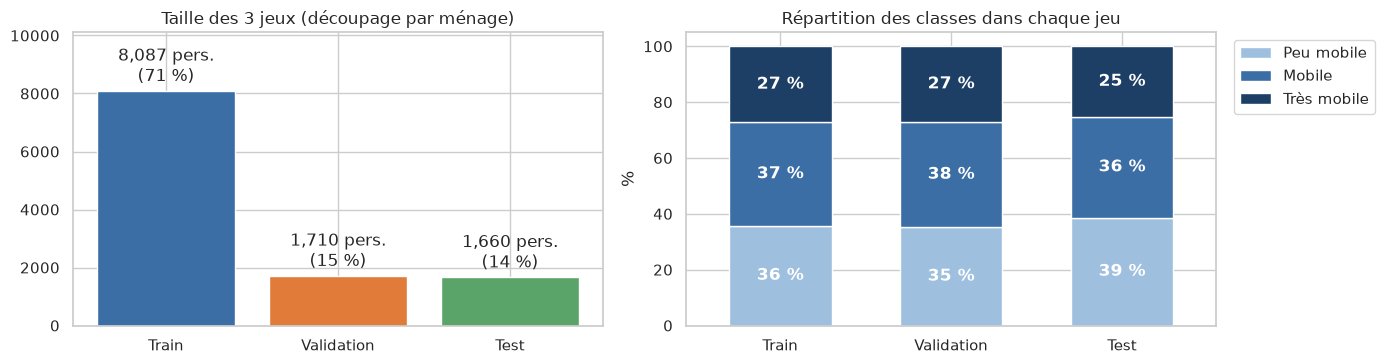
\includegraphics[width=\linewidth]{fig_split.png}
\caption{Taille des trois jeux et répartition des classes dans chacun}\label{fig:split}
\end{figure}

\section{Préparation des features}
Les modèles de Spark MLlib attendent une seule colonne contenant un vecteur de nombres. La préparation enchaîne :
\begin{itemize}[leftmargin=*]
  \item \code{StringIndexer}, qui transforme chaque variable texte en numéro ;
  \item \code{OneHotEncoder} (Logistic Regression uniquement), qui transforme ces numéros en colonnes 0/1 ;
  \item \code{VectorAssembler}, qui rassemble toutes les variables dans un vecteur \code{features} ;
  \item \code{StandardScaler} (Logistic Regression uniquement), qui met les variables à la même échelle.
\end{itemize}

\section{Modèles comparés}
Chaque modèle est placé dans un \code{Pipeline} MLlib avec les étapes de préparation, entraîné sur le train set (\code{fit}) et évalué sur le validation set (\code{transform}).
\begin{table}[H]
\centering
\caption{Modèles comparés, réglages de départ et valeurs testées}\label{tab:modeles}
\small
\begin{tabularx}{\linewidth}{@{}lXX@{}}
\toprule
\textbf{Modèle} & \textbf{Réglages de départ (étape 1)} & \textbf{Valeurs testées (étape 2)} \\
\midrule
Baseline & Prédit toujours la classe la plus fréquente du train set (\emph{mobile}) & -- \\
Logistic Regression & Multinomiale, 200 itérations, \code{regParam} = 0,01 & \code{regParam} : 0,001 ; 0,01 ; 0,1 ; 0,3 ; 1 \\
Decision Tree & \code{maxDepth} = 6 & \code{maxDepth} : 3 ; 5 ; 7 ; 9 ; 12 \\
Random Forest & 100 arbres, \code{maxDepth} = 10 & \code{maxDepth} : 6 ; 8 ; 10 \(\times\) \code{minInstancesPerNode} : 1 ; 5 \\
\bottomrule
\end{tabularx}
\end{table}

\section{Métriques d'évaluation}
\begin{itemize}[leftmargin=*]
  \item \textbf{Accuracy} : part des personnes correctement classées.
  \item \textbf{Recall par classe} : part des personnes d'une classe que le modèle retrouve (par exemple, la part des très mobiles reconnus comme très mobiles).
  \item \textbf{Weighted F1-score} : moyenne de la precision et du recall de chaque classe, pondérée par la taille des classes.
\end{itemize}

\section{Démarche de sélection en trois étapes}
\begin{enumerate}[leftmargin=*]
  \item \textbf{Comparer} les trois modèles dans les deux scénarios sur le validation set, avec leurs réglages de départ.
  \item \textbf{Régler les hyperparameters} de chaque modèle (scénario B) : chaque réglage est entraîné sur le train set et évalué sur le train set et sur le validation set ; on garde la meilleure accuracy de validation.
  \item \textbf{Évaluer une seule fois} le modèle retenu sur le test set.
\end{enumerate}

\begin{lstlisting}[caption={Réglage des hyperparameters sur le validation set},label={lst:reglage}]
grilles = {
    "Logistic Regression": [{"regParam": r} for r in [0.001, 0.01, 0.1, 0.3, 1.0]],
    "Decision Tree":       [{"maxDepth": d} for d in [3, 5, 7, 9, 12]],
    "Random Forest":       [{"maxDepth": d, "minInstancesPerNode": m}
                            for d in [6, 8, 10] for m in [1, 5]],
}
for nom, grille in grilles.items():
    for params in grille:
        modele = construire(nom, cat_B, **params).fit(train)
        acc_train = mc("accuracy").evaluate(modele.transform(train))
        acc_val = mc("accuracy").evaluate(modele.transform(valid))
\end{lstlisting}

\begin{attention}[Pourquoi pas de cross-validation~?]
Le \code{CrossValidator} de Spark découpe le train set \textbf{personne par personne} : des membres d'un même ménage se retrouvent dans des folds différents, ce qui rend le score trop optimiste. Le validation set, lui, est découpé \textbf{par ménage}, comme le test set.
\end{attention}

\section{Synthèse du chapitre}
Trois modèles sont comparés à une baseline naïve, dans deux scénarios de variables. Les choix (scénario, modèle, hyperparameters) sont faits sur le validation set, et le test set ne sert qu'à l'évaluation finale. Le découpage par ménage empêche le data leakage entre les trois jeux.

% ============================================================
% CHAPITRE 7 — RÉSULTATS
% ============================================================
\chapter{Résultats}\label{ch:resultats}

\section{Étape 1 : comparaison des modèles sur le validation set}
\begin{table}[H]
\centering
\caption{Performances sur le validation set (1\,710 individus), réglages de départ}\label{tab:resultats}
\small
\resizebox{\linewidth}{!}{%
\begin{tabular}{@{}llccccc@{}}
\toprule
\multirow{2}{*}{\textbf{Scénario}} & \multirow{2}{*}{\textbf{Modèle}} & \multirow{2}{*}{\textbf{Accuracy}} & \multirow{2}{*}{\textbf{Weighted F1}} & \multicolumn{3}{c}{\textbf{Recall}} \\
\cmidrule(l){5-7}
 & & & & Peu & Mobile & Très \\
\midrule
-- & Baseline (classe majoritaire) & 0,378 & 0,207 & 0,000 & 1,000 & 0,000 \\
\midrule
\multirow{3}{*}{A} & Logistic Regression & 0,424 & 0,421 & 0,518 & 0,387 & 0,353 \\
 & Decision Tree & 0,418 & 0,412 & 0,429 & 0,514 & 0,268 \\
 & Random Forest & 0,423 & 0,419 & 0,512 & 0,429 & 0,299 \\
\midrule
\multirow{3}{*}{B} & Logistic Regression & 0,441 & 0,438 & 0,542 & 0,410 & 0,353 \\
 & Decision Tree & 0,425 & 0,388 & 0,508 & 0,594 & 0,078 \\
 & \cellcolor{bleu!8}\textbf{Random Forest} & \cellcolor{bleu!8}\textbf{0,445} & \cellcolor{bleu!8}\textbf{0,437} & \cellcolor{bleu!8}0,525 & \cellcolor{bleu!8}0,500 & \cellcolor{bleu!8}0,264 \\
\bottomrule
\end{tabular}}
\end{table}

\begin{figure}[H]
\centering
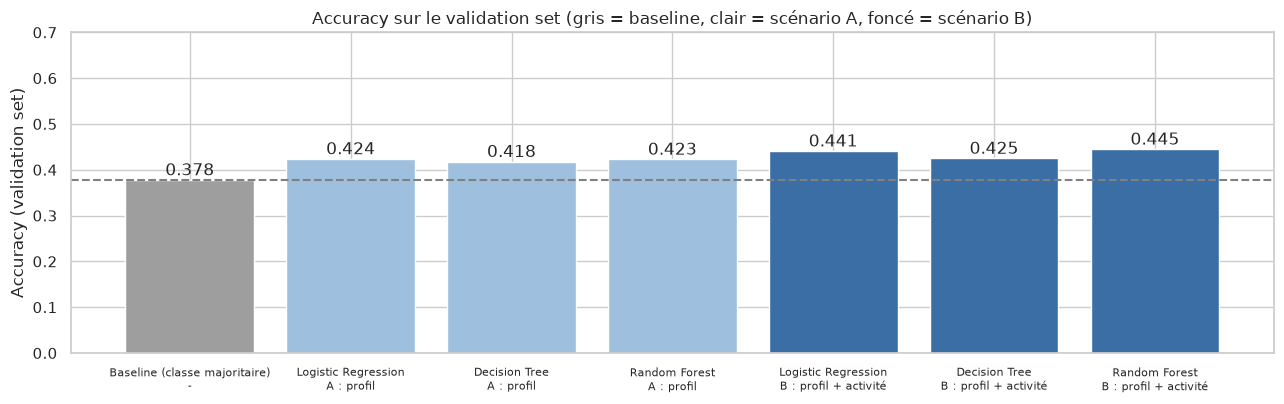
\includegraphics[width=0.95\linewidth]{fig_val_comparaison.png}
\caption{Accuracy sur le validation set (gris : baseline, clair : scénario A, foncé : scénario B)}\label{fig:comparaison}
\end{figure}

\begin{constat}[Lecture des résultats]
\begin{itemize}[leftmargin=*]
  \item Les six modèles battent la baseline (0,378).
  \item \textbf{Le scénario B fait mieux que le scénario A pour les trois modèles} : l'activité de la journée aide (Random Forest 0,423 \(\rightarrow\) 0,445 ; Logistic Regression 0,424 \(\rightarrow\) 0,441). On garde donc le scénario B.
  \item Les écarts entre modèles restent faibles (0,42 à 0,45). Le Decision Tree du scénario B ne reconnaît presque aucun très mobile (recall 0,078) : un seul arbre est instable.
\end{itemize}
\end{constat}

\section{Étape 2 : réglage des hyperparameters}
\begin{figure}[H]
\centering
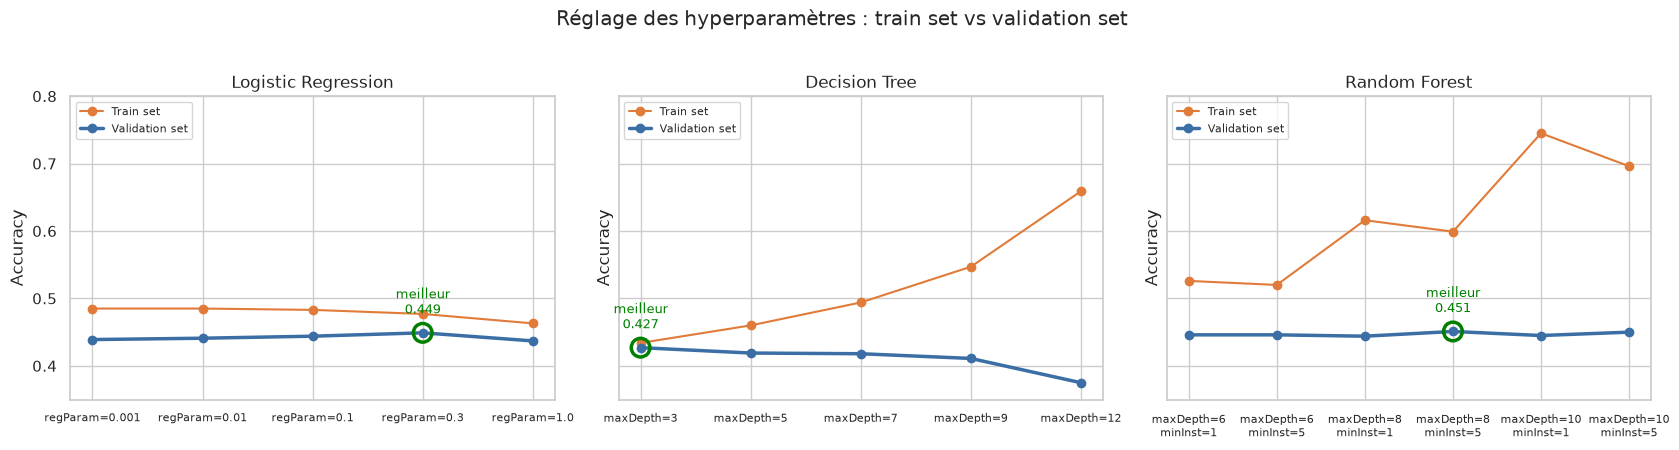
\includegraphics[width=\linewidth]{fig_reglage.png}
\caption{Accuracy sur le train set et sur le validation set selon les hyperparameters}\label{fig:reglage}
\end{figure}

La figure~\ref{fig:reglage} met en évidence l'\textbf{overfitting} :
\begin{itemize}[leftmargin=*]
  \item \textbf{Decision Tree} : plus l'arbre est profond, plus l'accuracy train monte (0,43 \(\rightarrow\) 0,66), mais l'accuracy de validation \textbf{baisse} (0,427 \(\rightarrow\) 0,375). L'arbre apprend par cœur les personnes du train set ; le meilleur réglage est le plus simple (\code{maxDepth} = 3).
  \item \textbf{Random Forest} : l'accuracy train monte aussi (0,52 \(\rightarrow\) 0,75), mais l'accuracy de validation reste stable autour de 0,45. En faisant voter 100 arbres différents, la forêt \textbf{résiste} à l'overfitting. Le meilleur réglage est \code{maxDepth} = 8, \code{minInstancesPerNode} = 5.
  \item \textbf{Logistic Regression} : train et validation restent proches (environ 0,48 et 0,44) ; un modèle linéaire a peu de risque d'overfitting. Une régularisation modérée (\code{regParam} = 0,3) aide un peu ; trop forte (1), elle dégrade le modèle.
\end{itemize}

\begin{table}[H]
\centering
\caption{Meilleur réglage de chaque modèle (scénario B)}\label{tab:reglage}
\small
\resizebox{\linewidth}{!}{%
\begin{tabular}{@{}llcc@{}}
\toprule
\textbf{Modèle} & \textbf{Meilleur réglage} & \textbf{Accuracy train} & \textbf{Accuracy validation} \\
\midrule
\cellcolor{bleu!8}\textbf{Random Forest} & \cellcolor{bleu!8}\code{maxDepth} = 8, \code{minInstancesPerNode} = 5 & \cellcolor{bleu!8}0,599 & \cellcolor{bleu!8}\textbf{0,451} \\
Logistic Regression & \code{regParam} = 0,3 & 0,477 & 0,449 \\
Decision Tree & \code{maxDepth} = 3 & 0,434 & 0,427 \\
\bottomrule
\end{tabular}}
\end{table}

Le Random Forest (0,451) et la Logistic Regression (0,449) sont \textbf{quasiment à égalité}. On applique la règle fixée à l'avance : le modèle retenu est celui qui a la meilleure accuracy de validation, le \textbf{Random Forest}.

\section{Étape 3 : évaluation finale sur le test set}
\begin{table}[H]
\centering
\caption{Performances sur le test set (1\,660 individus de ménages jamais vus)}\label{tab:test}
\small
\resizebox{\linewidth}{!}{%
\begin{tabular}{@{}lccccc@{}}
\toprule
\multirow{2}{*}{\textbf{Modèle}} & \multirow{2}{*}{\textbf{Accuracy}} & \multirow{2}{*}{\textbf{Weighted F1}} & \multicolumn{3}{c}{\textbf{Recall}} \\
\cmidrule(l){4-6}
 & & & Peu & Mobile & Très \\
\midrule
Baseline (classe majoritaire) & 0,361 & 0,192 & 0,000 & 1,000 & 0,000 \\
\cellcolor{bleu!8}\textbf{Random Forest} (\code{maxDepth} = 8, \code{minInstancesPerNode} = 5) & \cellcolor{bleu!8}\textbf{0,447} & \cellcolor{bleu!8}\textbf{0,440} & \cellcolor{bleu!8}0,520 & \cellcolor{bleu!8}0,500 & \cellcolor{bleu!8}0,258 \\
\bottomrule
\end{tabular}}
\end{table}

\begin{figure}[H]
\centering
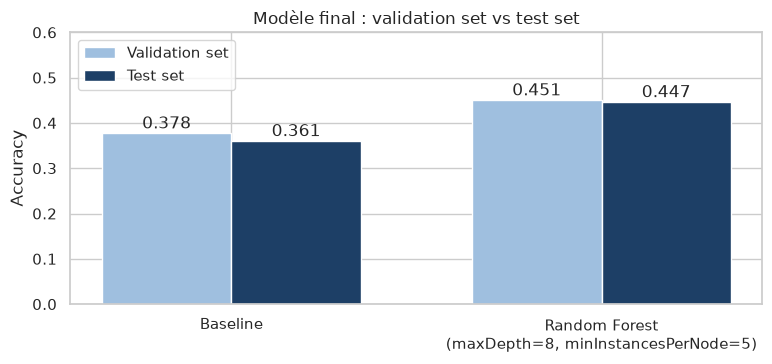
\includegraphics[width=0.62\linewidth]{fig_val_test.png}
\caption{Accuracy du modèle final et de la baseline sur le validation set et sur le test set}\label{fig:valtest}
\end{figure}

Le modèle final gagne \textbf{8,6 points} d'accuracy sur la baseline. Son accuracy de test (0,447) est très proche de celle de validation (0,451) : le score annoncé est \textbf{fiable}, le modèle ne s'est pas sur-adapté au validation set pendant les choix.

\section{Confusion matrix}
\begin{figure}[H]
\centering
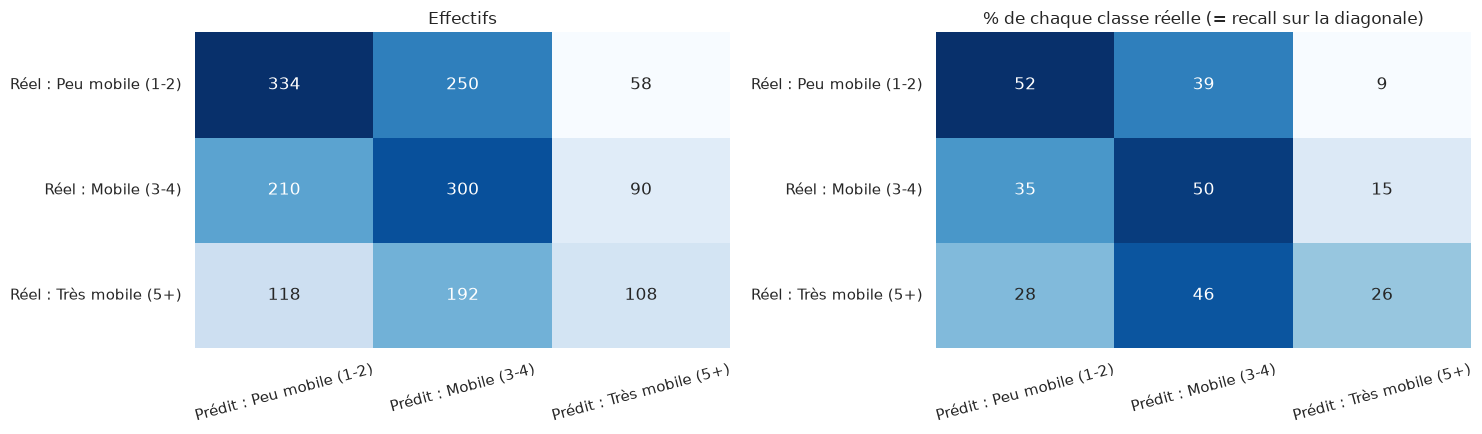
\includegraphics[width=\linewidth]{fig_confusion.png}
\caption{Confusion matrix du modèle final sur le test set (effectifs et pourcentages par classe réelle)}\label{fig:confusion}
\end{figure}

La confusion matrix (figure~\ref{fig:confusion}) montre que :
\begin{itemize}
  \item les classes \emph{peu mobile} (52\,\%) et \emph{mobile} (50\,\%) sont reconnues environ une fois sur deux ;
  \item la classe \emph{très mobile} est la plus difficile (26\,\%) : 46\,\% de ses membres sont prédits \emph{mobiles}, car rien dans le profil ne distingue une personne faisant 6 déplacements d'une personne en faisant 4 ;
  \item les erreurs portent surtout sur des \textbf{classes voisines}.
\end{itemize}

\section{Faux positifs et faux négatifs}
Avec trois classes, les faux positifs (FP) et faux négatifs (FN) sont calculés pour chaque classe, en la comparant aux deux autres (\emph{one-vs-rest}). Pour une classe donnée, un FN est une personne de cette classe que le modèle a classée ailleurs (reste de la ligne dans la confusion matrix), et un FP une personne classée à tort dans cette classe (reste de la colonne).

\begin{table}[H]
\centering
\caption{TP, FP, FN, precision et recall par classe (test set)}\label{tab:fpfn}
\small
\begin{tabular}{@{}lrrrrcc@{}}
\toprule
\textbf{Classe} & \textbf{TP} & \textbf{FP} & \textbf{FN} & \textbf{TN} & \textbf{Precision} & \textbf{Recall} \\
\midrule
Peu mobile & 334 & 328 & 308 & 690 & 0,505 & 0,520 \\
Mobile & 300 & 442 & 300 & 618 & 0,404 & 0,500 \\
Très mobile & 108 & 148 & 310 & 1\,094 & 0,422 & 0,258 \\
\bottomrule
\end{tabular}
\end{table}

\begin{figure}[H]
\centering
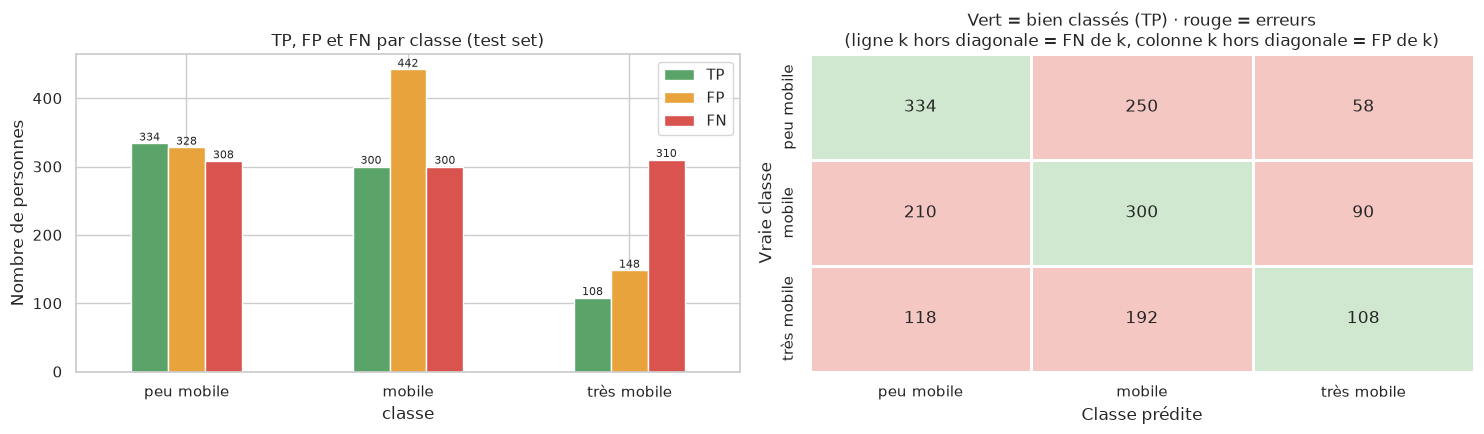
\includegraphics[width=\linewidth]{fig_fpfn.png}
\caption{TP, FP et FN par classe, et confusion matrix colorée (vert : bien classés, rouge : erreurs)}\label{fig:fpfn}
\end{figure}

\begin{constat}[Lecture]
\begin{itemize}[leftmargin=*]
  \item \textbf{Très mobile} : beaucoup de FN (310) pour peu de TP (108). Le modèle \textbf{rate 3 très mobiles sur 4}, mais quand il prédit « très mobile », il a raison dans 42\,\% des cas : il est prudent et prédit rarement cette classe.
  \item \textbf{Mobile} : le plus de FP (442). C'est la classe « du milieu » : quand le modèle hésite, il répond souvent « mobile ».
  \item \textbf{Peu mobile} : la classe la plus équilibrée (precision 0,51, recall 0,52). Le modèle est donc plus utile pour repérer les personnes peu mobiles que les très mobiles.
\end{itemize}
\end{constat}

\section{Feature importance}
\begin{figure}[H]
\centering
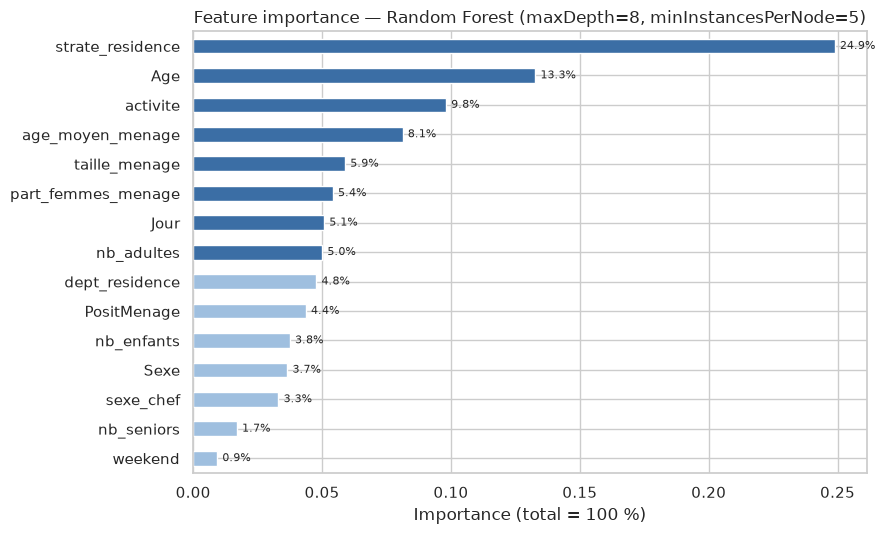
\includegraphics[width=0.75\linewidth]{fig_importance.png}
\caption{Feature importance du Random Forest retenu}\label{fig:importance}
\end{figure}

La \textbf{zone de résidence} (25\,\%) arrive en tête, suivie de l'\textbf{âge} (13\,\%), de l'\textbf{activité} (10\,\%) et de l'\textbf{âge moyen du ménage} (8\,\%). Le jour et le week-end comptent très peu, ce qui confirme l'EDA. La feature importance de la strate de résidence est toutefois surestimée : les Random Forests favorisent les variables catégorielles à nombreuses modalités.

\section{Analyse des erreurs}
\begin{figure}[H]
\centering
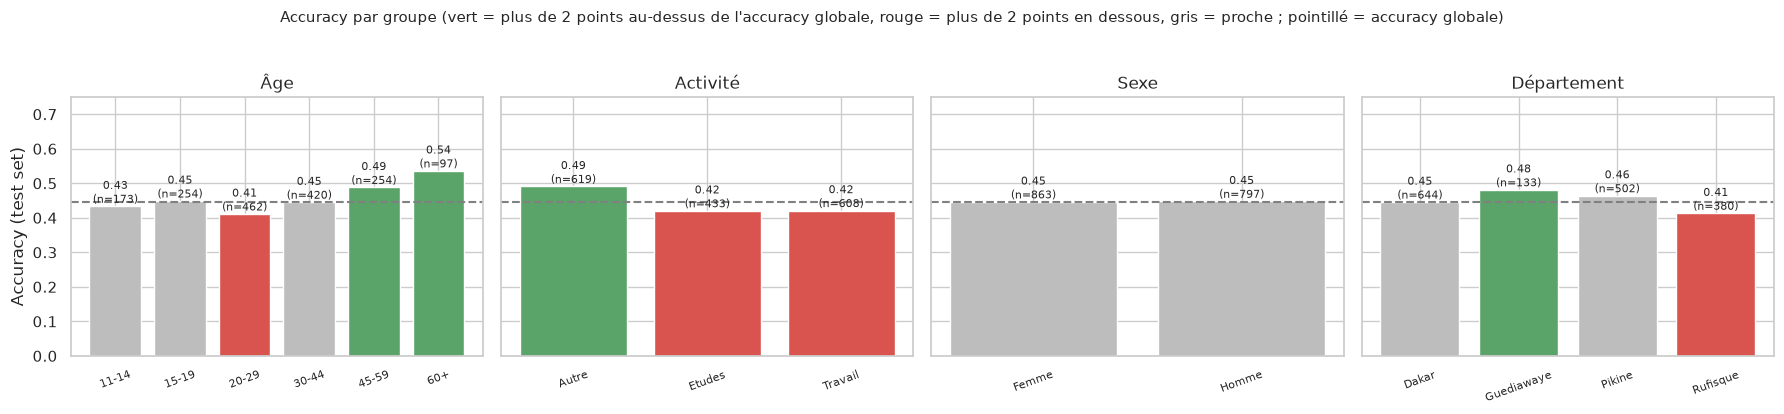
\includegraphics[width=\linewidth]{fig_erreurs.png}
\caption{Accuracy du modèle final selon le profil (test set)}\label{fig:erreurs}
\end{figure}

Le modèle prédit mieux les \textbf{plus de 45 ans} (0,49 à 0,54) et les personnes \textbf{sans travail ni études} ce jour-là (0,49), dont le comportement est plus régulier. Il se trompe davantage pour les \textbf{20--29 ans} (0,41), les \textbf{élèves et les actifs} (0,42) et les habitants de \textbf{Rufisque} (0,41), dont la mobilité dépend d'éléments non observés (type d'emploi, horaires, distances). Il n'y a \textbf{aucune différence selon le sexe} (0,45 pour les hommes comme pour les femmes).

\section{Confiance du modèle}
\begin{figure}[H]
\centering
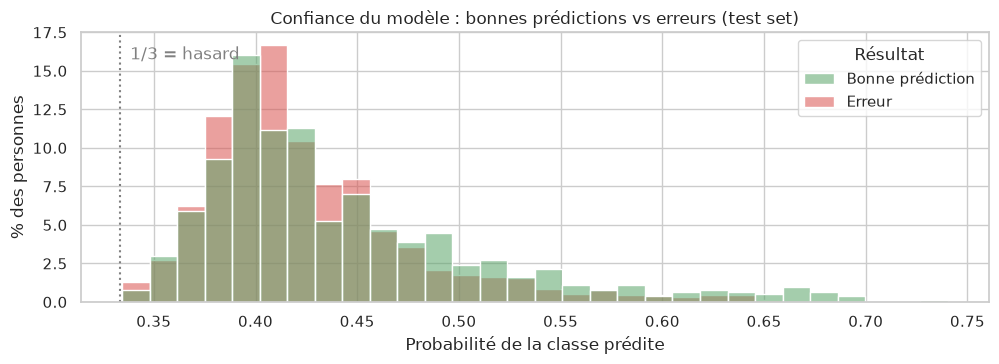
\includegraphics[width=0.8\linewidth]{fig_confiance.png}
\caption{Probabilité de la classe prédite pour les bonnes prédictions et pour les erreurs}\label{fig:confiance}
\end{figure}

Les probabilités de la classe prédite sont presque toutes comprises entre 0,35 et 0,50, à peine au-dessus du hasard (1/3) : le modèle est \textbf{rarement sûr de lui}. Les distributions des bonnes prédictions et des erreurs se recouvrent presque entièrement (médianes 0,42 et 0,41) ; ce n'est qu'au-delà de 0,55 que les bonnes prédictions dominent.

\section{Exemple d'utilisation du modèle}
Le modèle final est appliqué à des profils fictifs, créés directement en Spark SQL (tableau~\ref{tab:exemples} et figure~\ref{fig:nouveaux}).

\begin{table}[H]
\centering
\caption{Prédictions pour quatre profils fictifs}\label{tab:exemples}
\small
\resizebox{\linewidth}{!}{%
\begin{tabular}{@{}rllllc@{}}
\toprule
\textbf{Âge} & \textbf{Sexe} & \textbf{Activité} & \textbf{Résidence} & \textbf{Niveau prédit} & \textbf{Probabilités (peu / mobile / très)} \\
\midrule
14 & Homme & Études & Guédiawaye & Très mobile & 0,15 / 0,33 / \textbf{0,52} \\
35 & Femme & Autre & Dakar & Peu mobile & \textbf{0,42} / 0,41 / 0,17 \\
40 & Homme & Travail & Pikine & Peu mobile & \textbf{0,39} / 0,36 / 0,25 \\
67 & Femme & Autre & Rufisque & Peu mobile & \textbf{0,55} / 0,32 / 0,13 \\
\bottomrule
\end{tabular}}
\end{table}

\begin{figure}[H]
\centering
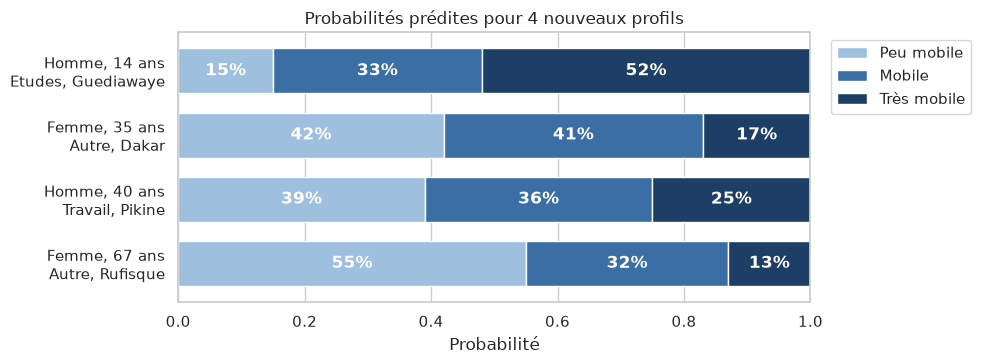
\includegraphics[width=0.8\linewidth]{fig_nouveaux.png}
\caption{Probabilités prédites pour quatre nouveaux profils}\label{fig:nouveaux}
\end{figure}

Les profils typés sont nettement classés (l'élève de 14 ans est « très mobile », la femme de 67 ans « peu mobile »), alors que le modèle \textbf{hésite} pour les profils « moyens » (42\,\% contre 41\,\% pour la femme de 35 ans), exactement ceux où il se trompe le plus.

\section{Synthèse du chapitre}
Le modèle retenu, un Random Forest, atteint 44,7\,\% d'accuracy sur le test set contre 36,1\,\% pour la baseline, un score proche de celui de validation. Les courbes de réglage montrent l'overfitting du Decision Tree et la robustesse du Random Forest. Les erreurs portent surtout sur des classes voisines, et la classe \emph{très mobile}, avec beaucoup de faux négatifs, est la plus difficile à reconnaître.

% ============================================================
% CHAPITRE 8 — DISCUSSION
% ============================================================
\chapter{Discussion}\label{ch:discussion}

\section{Interprétation}
Les résultats confirment les grandes tendances connues de la mobilité dans les villes d'Afrique de l'Ouest :
\begin{itemize}
  \item une \textbf{mobilité scolaire} très intense, avec des allers-retours multiples dans la journée ;
  \item une \textbf{inégalité de genre} : les femmes adultes, et en particulier celles sans activité de travail ou d'études, se déplacent moins ;
  \item une \textbf{mobilité plus élevée en banlieue} (Rufisque, Guédiawaye) qu'à Dakar ville, où les équipements sont plus proches.
\end{itemize}

La performance modeste du modèle est elle-même un résultat : \textbf{le profil socio-démographique n'explique qu'une partie de la mobilité individuelle}. Deux personnes au profil identique peuvent avoir des journées très différentes. Le fait que le Random Forest et la Logistic Regression atteignent presque le même score, et que le réglage des hyperparameters ne change presque rien, confirme que la limite vient \textbf{des données et non de l'algorithme}.

\section{Limites}
\begin{enumerate}
  \item \textbf{Variables manquantes} : le revenu, la profession, la possession d'un véhicule et la distance aux lieux d'activité, déterminants connus de la mobilité, ne figurent pas dans les données. C'est la principale limite.
  \item \textbf{Absence d'individus immobiles} : la target ne couvre pas le cas « 0 déplacement ».
  \item \textbf{Activité déduite} : dans le scénario B, l'activité est tirée des motifs de la journée et non déclarée ; elle doit être vue comme un indicateur de statut.
  \item \textbf{Une seule journée observée} par individu : la variabilité d'un jour à l'autre n'est pas mesurée.
\end{enumerate}

\section{Bonnes pratiques Big Data mises en œuvre}
\begin{table}[H]
\centering
\caption{Bonnes pratiques Big Data appliquées}\label{tab:pratiques}
\small
\begin{tabularx}{\linewidth}{@{}lX@{}}
\toprule
\textbf{Pratique} & \textbf{Mise en œuvre} \\
\midrule
Schéma explicite & 33 champs typés, aucun \code{inferSchema} sur la table principale \\
Mise en cache & \code{cache()} des tables réutilisées (nettoyée, individus, train, validation et test sets) \\
Agrégation distribuée & \code{groupBy} déplacements \(\rightarrow\) individus, \code{max\_by} \\
Fonctions de fenêtre & Variables de ménage sans jointure ni collecte \\
Collecte minimale & Seuls les petits résultats agrégés sont convertis en pandas \\
Pipelines MLlib & Encodage et modèle dans un même \code{Pipeline} reproductible \\
Sélection de modèle & Choix du scénario, du modèle et des hyperparameters sur le validation set ; test set utilisé une seule fois \\
Prévention du data leakage & Split train / validation / test par ménage, exclusion des variables issues de la journée \\
Réutilisation du modèle & \code{PipelineModel} complet appliqué à de nouveaux profils \\
\bottomrule
\end{tabularx}
\end{table}


% ============================================================
% CONCLUSION GÉNÉRALE
% ============================================================
\chapter*{Conclusion générale}
\addcontentsline{toc}{chapter}{Conclusion générale}

Ce projet a permis de construire une chaîne complète de traitement Big Data, de l'EDA à la modélisation distribuée, sur l'enquête ménages-déplacements de Dakar. L'EDA a guidé chacune des décisions de préparation : correction des heures et des codes, choix de la zone de résidence, définition de la target et exclusion des variables sources de data leakage.

Sur le plan thématique, l'étude montre qu'un Dakarois mobile réalise en moyenne \textbf{3,9 déplacements par jour}, que les jeunes, les élèves, les hommes et les habitants de la banlieue sont les plus mobiles, et que les journées s'organisent en allers-retours depuis le domicile. Sur le plan prédictif, après un découpage train / validation / test (70 / 15 / 15) par ménage, le modèle retenu (Random Forest) atteint une accuracy de \textbf{44,7\,\%} sur le test set, contre 36,1\,\% pour la baseline : le profil d'une personne renseigne sur sa mobilité, mais n'en explique qu'une partie. La classe des personnes très mobiles reste la plus difficile à repérer.

\paragraph{Perspectives.}
\begin{itemize}[leftmargin=*]
  \item Modéliser directement le nombre de déplacements par une \textbf{régression de Poisson} (\code{GeneralizedLinearRegression}).
  \item Réduire la target à \textbf{deux classes} (peu mobile / mobile), une tâche plus facile.
  \item Prédire le \textbf{type de journée} (chaîne domicile $\rightarrow$ travail $\rightarrow$ domicile, domicile $\rightarrow$ école $\rightarrow$ marché $\rightarrow$ domicile, etc.).
  \item Enrichir les données par des sources externes (recensement, revenu, motorisation des ménages, distances réelles) afin de lever la principale limite identifiée.
  \item Déployer le pipeline sur un cluster Spark pour traiter plusieurs vagues d'enquête ou des données de traces numériques.
\end{itemize}

% ============================================================
% ANNEXES
% ============================================================
\appendix
\titleformat{\chapter}[display]
  {\normalfont\Large\bfseries\color{ReportBlueDark}}
  {\filleft\large\color{ReportGold}Annexe \thechapter}
  {1ex}
  {\titlerule[1.4pt]\vspace{1ex}\filright}
  [\vspace{0.8ex}\titlerule]
\chapter{Dictionnaire des variables construites}
\begin{table}[H]
\centering
\caption{Variables créées au niveau individu}\label{tab:dico}
\small
\begin{tabularx}{\linewidth}{@{}lX@{}}
\toprule
\textbf{Variable} & \textbf{Définition} \\
\midrule
\code{nb\_dep} & Nombre de déplacements de l'individu dans la journée \\
\code{niveau} & Cible : 0 (1--2 déplacements), 1 (3--4), 2 (5 et plus) \\
\code{strate\_residence} & Strate d'arrivée du dernier déplacement de la journée \\
\code{dept\_residence} & Département déduit de la strate (Dakar, Pikine, Guédiawaye, Rufisque, Extérieur, Inconnu) \\
\code{activite} & Travail si un motif de travail, sinon Études si un motif d'études, sinon Autre \\
\code{taille\_menage} & Nombre de personnes mobiles du ménage \\
\code{nb\_enfants}, \code{nb\_adultes}, \code{nb\_seniors} & Membres de moins de 18 ans, de 18 à 59 ans, de 60 ans et plus \\
\code{age\_moyen\_menage} & Âge moyen des membres du ménage \\
\code{part\_femmes\_menage} & Proportion de femmes dans le ménage \\
\code{sexe\_chef} & Sexe du chef de ménage \\
\code{weekend} & 1 si l'enquête porte sur un samedi ou un dimanche \\
\code{poids} & Poids d'extrapolation de l'individu \\
\bottomrule
\end{tabularx}
\end{table}

\chapter{Règle de calcul du département}
\begin{lstlisting}[caption={Département à partir du code de strate, codes spéciaux inclus},label={lst:dept}]
dept_map = F.create_map([F.lit(x) for x in
    ["D", "Dakar", "P", "Pikine", "G", "Guediawaye", "R", "Rufisque"]])

def departement(col):
    return (F.when(col == "zex", "Exterieur")             # hors zone d'étude
             .when(col == "NA_region", "Inconnu")          # localisation inconnue
             .when(col.startswith("NA"),                   # NA_d, NA_p, NA_g, NA1_r
                   dept_map[F.upper(F.substring_index(col, "_", -1))])
             .otherwise(dept_map[F.substring(col, 1, 1)]))  # D05 -> Dakar
\end{lstlisting}

Le code complet est fourni dans le notebook {\small\nolinkurl{Projet_BigData_Niveau_Mobilite_Dakar.ipynb}}.

\end{document}
